\subsection{Our Parallel Naive-dynamic (ND) Louvain}
\label{sec:our-naive}

Algorithm \ref{alg:naive} presents our multicore implementation of Naive dynamic (ND) Louvain, where vertices are assigned to communities from the previous snapshot of the graph, and all vertices are processed irrespective of edge deletions and insertions in the batch update. Algorithm \ref{alg:naive} requires several inputs, including the previous $G^{t-1}$ and current graph snapshots $G^t$, edge deletions $\Delta^{t-}$ and insertions $\Delta^{t+}$ in the batch update, the previous community membership of each vertex $C^{t-1}$, weighted degree of each vertex $K^{t-1}$, and total edge weight of each community $\Sigma^{t-1}$. The output consists of the updated community memberships $C^t$, weighted-degrees $K^t$, and total edge weight of communities $\Sigma^t$.

In the algorithm, we start by defining two lambda functions for the Louvain algorithm, \texttt{isAffected()} (lines \ref{alg:naive--isaff-begin}-\ref{alg:naive--isaff-end}) and \texttt{inAffectedR} \texttt{ange()} (lines \ref{alg:naive--isaffrng-begin}-\ref{alg:naive--isaffrng-end}), which indicate that all vertices in the graph $G^t$ are to be marked as affected, and that all such vertices can be incrementally marked as affected, respectively. Unlike existing works, we then utilize $K^{t-1}$ and $\Sigma^{t-1}$, along with the batch update $\Delta^{t-}$ and $\Delta^{t+}$, to quickly obtain $K^t$ and $\Sigma^t$ which is needed in the local-moving phase of the Louvain algorithm (line \ref{alg:naive--auxliliary}). The lambda functions and the total vertex/edge weights are then used to run the Louvain algorithm, and obtain the updated community assignments $C^t$ (line \ref{alg:naive--louvain}). Finally, $C^t$ is returned, along with $K^t$ and $\Sigma^t$ as the updated auxiliary information (line \ref{alg:naive--return}).




\subsection{Our Parallel Delta-screening (DS) Louvain}
\label{sec:our-delta}

The pseudocode of our multicore implementation of Delta-screening (DS) Louvain is given in Algorithm \ref{alg:delta}. It uses modularity-based scoring to determine an approximate region of the graph in which vertices are likely to change their community membership \cite{com-zarayeneh21}. The algorithm accepts as input the previous $G^{t-1}$ and current snapshot of the graph $G^t$, edge deletions $\Delta^{t-}$ and insertions $\Delta^{t+}$ in the batch update, the previous community memberships of vertices $C^{t-1}$, weighted degrees of vertices $K^{t-1}$, and total edge weights of communities $\Sigma^{t-1}$. It outputs the updated community memberships $C^t$, weighted-degrees $K^t$, and total edge weights of communities $\Sigma^t$. The batch update, comprising edge deletions $(i, j, w) \in \Delta^{t-}$ and insertions $(i, j, w) \in \Delta^{t+}$, is sorted separately by their source vertex ID $i$ beforehand, as a preprocessing step.

\begin{algorithm}[hbtp]
\caption{\textit{Naive-dynamic} community detection approach.}
\label{alg:naive}
\begin{algorithmic}
\Ensure{$communities$: Community detection algorithm to use.}

\Statex

\Function{naiveDynamic}{$G^{t-1}, C^{t-1}, \Delta^{t-}, \Delta^{t+}$}
  \State $G^t \gets G^{t-1} \setminus \Delta^{t-} \cup \Delta^{t+}$
  \Function{isAffected}{$i$}
    \Return{$true$}
  \EndFunction
  \Return{$communities(G^t, C^{t-1}, \{isAffected\})$}
\EndFunction
\end{algorithmic}
\end{algorithm}

\begin{algorithm}[hbtp]
\caption{\textit{Dynamic $\Delta$-screening} community detection approach.}
\label{alg:dynamic-delta-screening}
\begin{algorithmic}
\Ensure{$\delta V, \delta E, \delta C$: Is vertex, neighbors, or community affected?}
\Ensure{$H$: Hashtable that maps a community to associated weight}
\Ensure{$communities$: Community detection algorithm to use.}

\Statex

\Function{dynamicDeltaScreening}{$G^{t-1}, C^{t-1}, \Delta^{t-}, \Delta^{t+}$}
  \State $G^t \gets G^{t-1} \setminus \Delta^{t-} \cup \Delta^{t+}$
  \State $\delta V \gets deltaScreeningAffected(G^{t-1}, C^{t-1}, \Delta^{t-}, \Delta^{t+})$
  \Function{isAffected}{$i$}
    \Return{$\delta V[i]$}
  \EndFunction
\Return{$communities(G^t, C^{t-1}, isAffected)$}
\EndFunction

\Statex

\Function{deltaScreeningAffected}{$G^{t-1}, C^{t-1}, \Delta^{t-}, \Delta^{t+}$}
  \State $H, \delta V, \delta E, \delta C \gets \{\}$
  \ForAll{$[i, j] \in \Delta^{t-}$}
    \If{$C^{t-1}[i] = C^{t-1}[j]$}
      \State $\delta V[i], \delta E[i], \delta C[C^{t-1}[j]] \gets true$
    \EndIf
  \EndFor
  \ForAll{$i \in uniqueFrom(\Delta^{t+})$}
    \State $H \gets \{\}$
    \ForAll{$[j, w] \in withFrom(\Delta^{t+}, i)$}
      \If{$C^{t-1}[i] \neq C^{t-1}[j]$}
        \State $H[C^{t-1}[j]] \gets H[C^{t-1}[j]] + w$
      \EndIf
    \EndFor
    \State $[c_{top}, w_{top}] \gets chooseCommunity(H)$
    \State $\delta V[i], \delta E[i], \delta C[c_{top}] \gets true$
  \EndFor
  \ForAll{$i \in G^{t-1}.vertices()$}
    \If{$\delta E[i]$}
      \ForAll{$j \in G^{t-1}.neighbors(i)$}
        \State $\delta V[j] \gets true$
      \EndFor
    \EndIf
    \If{$\delta C[C^{t-1}[i]]$}
      \State $\delta V[i] \gets true$
    \EndIf
  \EndFor
  \Return{$\delta V$}
\EndFunction
\end{algorithmic}
\end{algorithm}


In the algorithm, we first initialize a hashtable $H$, mapping communities to their associated weights, and affected flags $\delta V$, $\delta E$, and $\delta C$, indicating if a vertex, its neighbors, or its community is affected by the batch update (lines \ref{alg:delta--init}). Then, we parallelly iterate over edge deletions $\Delta^{t-}$ and insertions $\Delta^{t+}$. For each deletion $(i, j, w) \in \Delta^{t-}$ where $i$ and $j$ are in the same community, we mark the source vertex $i$, its neighbors, and its community as affected (lines \ref{alg:delta--loopdel-begin}-\ref{alg:delta--loopdel-end}). For each unique source vertex $i\ |\ (i, j, w) \in \Delta^{t+}$ in insertions belonging to different communities, we identify the community $c^*$ with the highest delta-modularity if $i$ moves to one of its neighboring communities and mark $i$, its neighbors, and the community $c^*$ as affected (lines \ref{alg:delta--loopins-begin}-\ref{alg:delta--loopins-end}). Deletions between different communities and insertions within the same community are disregarded. Using affected neighbor $\delta E$ and community flags $\delta C$, affected vertices in $\delta V$ are marked (lines \ref{alg:delta--loopaff-begin}-\ref{alg:delta--loopaff-end}). Next, similar to ND Louvain, we use $K^{t-1}$ and $\Sigma^{t-1}$, along with $\Delta^{t-}$ and $\Delta^{t+}$, to quickly yield $K^t$ and $\Sigma^t$ (line \ref{alg:naive--auxliliary}), define the needed lambda functions \texttt{isAffected()} (lines \ref{alg:delta--isaff-begin}-\ref{alg:delta--isaff-end}) and \texttt{inAffectedRange()} (lines \ref{alg:delta--isaffrng-begin}-\ref{alg:delta--isaffrng-end}), and run the Louvain algorithm, yielding updated community assignments $C^t$ (line \ref{alg:delta--louvain}). Finally, updated community memberships $C^t$ are returned, alongside $K^t$ and $\Sigma^t$ as updated auxiliary information (line \ref{alg:delta--return}).




\subsection{Our Dynamic-supporting Parallel Louvain}
\label{sec:our-louvain}

The main step of our Dynamic-supporting Parallel Louvain algorithm is given in Algorithm \ref{alg:louvain}. Unlike our implementation of Static Louvain \cite{sahu2023gvelouvain}, in addition to the current graph snapshot $G^t$, it accepts as input the previous community membership of each vertex $C^{t-1}$, the updated weighted-degree of each vertex $K^t$, the updated total edge weight of each community $\Sigma^t$, and a set of lambda functions $F$ which determine if a given vertex is affected, or if it can be incrementally marked as affected (it is in the affected range). It outputs the updated community memberships of vertices $C^t$.

\begin{algorithm}[hbtp]
\caption{GVE-Louvain: Our parallel Louvain algorithm.}
\label{alg:louvain}
\begin{algorithmic}[1]
\Require{$G$: Input graph}
\Require{$C$: Community membership of each vertex}
\Require{$G'$: Input/super-vertex graph}
\Require{$C'$: Community membership of each vertex in $G'$}
\Require{$K'$: Total edge weight of each vertex}
\Require{$\Sigma'$: Total edge weight of each community}
\Ensure{$G'_{C'}$: Community vertices (CSR)}
\Ensure{$H_t$: Collision-free per-thread hashtable}
\Ensure{$l_i$: Number of iterations performed (per pass)}
\Ensure{$l_p$: Number of passes performed}
\Ensure{$\tau$: Per iteration tolerance}
\Ensure{$\tau_{agg}$: Aggregation tolerance}

\Statex

\Function{louvain}{$G$} \label{alg:louvain--begin}
  \State Vertex membership: $C \gets [0 .. |V|)$ \textbf{;} $G' \gets G$ \label{alg:louvain--initialization}
  \ForAll{$l_p \in [0 .. \text{\small{MAX\_PASSES}})$} \label{alg:louvain--passes-begin}
    \State $\Sigma' \gets K' \gets vertexWeights(G')$ \textbf{;} $C' \gets [0 .. |V'|)$ \label{alg:louvain--reset-weights}
    \State Mark all vertices in $G'$ as unprocessed \label{alg:louvain--reset-affected}
    \State $l_i \gets louvainMove(G', C', K', \Sigma')$ \label{alg:louvain--local-move}
    \If{$l_i \le 1$} \textbf{break} \Comment{Globally converged?} \label{alg:louvain--globally-converged}
    \EndIf
    \State $|\Gamma|, |\Gamma_{old}| \gets$ Number of communities in $C$, $C'$
    \If{$|\Gamma|/|\Gamma_{old}| > \tau_{agg}$} \textbf{break} \Comment{Low shrink?} \label{alg:louvain--aggregation-tolerance}
    \EndIf
    \State $C' \gets$ Renumber communities in $C'$ \label{alg:louvain--renumber}
    \State $C \gets$ Lookup dendrogram using $C$ to $C'$ \label{alg:louvain--lookup}
    \State $G' \gets louvainAggregate(G', C')$ \label{alg:louvain--aggregate}
    \State $\tau \gets \tau / \text{\small{TOLERANCE\_DROP}}$ \Comment{Threshold scaling} \label{alg:louvain--threshold-scaling}
  \EndFor \label{alg:louvain--passes-end}
  \State $C \gets$ Lookup dendrogram using $C$ to $C'$ \label{alg:louvain--lookup-last}
  \Return{$C$} \label{alg:louvain--return}
\EndFunction \label{alg:louvain--end}
\end{algorithmic}
\end{algorithm}


In the algorithm, we commence by marking affected vertices as unprocessed (lines \ref{alg:louvain--mark-begin}-\ref{alg:louvain--mark-end}). Subsequently, the initialization phase follows, wherein we initialize the community membership of each vertex $C$ in $G^t$. Additionally, we initialize the total edge weight of each vertex $K'$, the total edge weight of each community $\Sigma'$, and the community membership $C'$ of each vertex in the current/super-vertex graph $G'$ (lines \ref{alg:louvain--init-begin}-\ref{alg:louvain--init-end}). After initialization, we conduct a series of passes (lines \ref{alg:louvain--passes-begin}-\ref{alg:louvain--passes-end}) of the local-moving and aggregation phases (limited to $MAX\_PASSES$). Within each pass, in line \ref{alg:louvain--local-move}, we execute the local-moving phase of the Louvain algorithm (Algorithm \ref{alg:louvainlm}), which optimizes community assignments. If the local-moving phase converges within a single iteration, it implies global convergence, prompting the termination of passes (line \ref{alg:louvain--globally-converged}). Conversely, if the drop in community count $|\Gamma|$ is deemed insignificant, indicating diminishing returns, we halt at the current pass (line \ref{alg:louvain--aggregation-tolerance}). Should the convergence conditions not be met, we progress to the aggregation phase. Here, we renumber communities (line \ref{alg:louvain--renumber}), update top-level community memberships $C$ using dendrogram lookup (line \ref{alg:louvain--lookup}), execute the aggregation phase (Algorithm \ref{alg:louvainag}), and adjust the convergence threshold for subsequent passes, i.e., perform threshold scaling (line \ref{alg:louvain--threshold-scaling}). The subsequent pass commences in line \ref{alg:louvain--passes-begin}. Following all passes, we do a final update of the top-level community membership $C$ of each vertex in $G^t$ via dendrogram lookup (line \ref{alg:louvain--lookup-last}), before ultimately returning it (line \ref{alg:louvain--return}).


\subsubsection{Local-moving phase of our Parallel Louvain}

The pseudocode detailing the local-moving phase of our Parallel Louvain algorithm is presented in Algorithm \ref{alg:louvainlm}. This phase iteratively moves vertices among communities in order to maximize modularity. Here, the \texttt{louvainMove()} function operates on the current graph $G'$, community membership $C'$, total edge weight of each vertex $K'$, total edge weight of each community $\Sigma'$, and a set of lambda functions as inputs, yielding the number of iterations performed $l_i$.

\begin{algorithm}[hbtp]
\caption{Local-moving phase of our Parallel Louvain \cite{sahu2023gvelouvain}.}
\label{alg:louvainlm}
\begin{algorithmic}[1]
\Require{$G'$: Input/super-vertex graph}
\Require{$C'$: Community membership of each vertex}
\Require{$K'$: Total edge weight of each vertex}
\Require{$\Sigma'$: Total edge weight of each community}
\Require{$F$: Lambda functions passed to parallel Louvain}
\Ensure{$H_t$: Collision-free per-thread hashtable}
\Ensure{$l_i$: Number of iterations performed}
\Ensure{$\tau$: Per iteration tolerance}

\Statex

\Function{louvainMove}{$G', C', K', \Sigma', F$} \label{alg:louvainlm--move-begin}
  \ForAll{$l_i \in [0 .. \text{\small{MAX\_ITERATIONS}})$} \label{alg:louvainlm--iterations-begin}
    \State Total delta-modularity per iteration: $\Delta Q \gets 0$ \label{alg:louvainlm--init-deltaq}
    \ForAll{unprocessed $i \in V'$ \textbf{in parallel}} \label{alg:louvainlm--loop-vertices-begin}
      \State Mark $i$ as processed (prune) \label{alg:louvainlm--prune}
      \If{\textbf{not} $F.inAffectedRange(i)$} \textbf{continue} \label{alg:louvainlm--affrng}
      \EndIf
      \State $H_t \gets scanCommunities(\{\}, G', C', i, false)$ \label{alg:louvainlm--scan}
      \State $\rhd$ Use $H_t, K', \Sigma'$ to choose best community
      \State $c^* \gets$ Best community linked to $i$ in $G'$ \label{alg:louvainlm--best-community-begin}
      \State $\delta Q^* \gets$ Delta-modularity of moving $i$ to $c^*$ \label{alg:louvainlm--best-community-end}
      \If{$c^* = C'[i]$} \textbf{continue} \label{alg:louvainlm--best-community-same}
      \EndIf
      \State $\Sigma'[C'[i]] -= K'[i]$ \textbf{;} $\Sigma'[c^*] += K'[i]$ \textbf{atomic} \label{alg:louvainlm--perform-move-begin}
      \State $C'[i] \gets c^*$ \textbf{;} $\Delta Q \gets \Delta Q + \delta Q^*$ \label{alg:louvainlm--perform-move-end}
      \State Mark neighbors of $i$ as unprocessed \label{alg:louvainlm--remark}
    \EndFor \label{alg:louvainlm--loop-vertices-end}
    \If{$\Delta Q \le \tau$} \textbf{break} \Comment{Locally converged?} \label{alg:louvainlm--locally-converged}
    \EndIf
  \EndFor \label{alg:louvainlm--iterations-end}
  \Return{$l_i$} \label{alg:louvainlm--return}
\EndFunction \label{alg:louvainlm--move-end}

\Statex

\Function{scanCommunities}{$H_t, G', C', i, self$}
  \ForAll{$(j, w) \in G'.edges(i)$}
    \If{$self$ \textbf{or} $i \neq j$} $H_t \gets H_t[C'[j]] + w$
    \EndIf
  \EndFor
  \Return{$H_t$}
\EndFunction
\end{algorithmic}
\end{algorithm}




%% Parameter setting
% $\tau \gets TOLERANCE\_INITIAL$
% TOLERANCE\_INITIAL = 0.01
% TOLERANCE\_DECLINE = 10
% MAX\_PASSES = 500


Lines \ref{alg:louvainlm--iterations-begin}-\ref{alg:louvainlm--iterations-end} encapsulate the primary loop of the local-moving phase. In line \ref{alg:louvainlm--init-deltaq}, we initialize the total delta-modularity per iteration $\Delta Q$. Subsequently, in lines \ref{alg:louvainlm--loop-vertices-begin}-\ref{alg:louvainlm--loop-vertices-end}, we concurrently iterate over unprocessed vertices. For each vertex $i$, we perform vertex pruning by marking $i$ as processed (line \ref{alg:louvainlm--prune}). Next, we verify if $i$ falls within the affected range (i.e., it is permitted to be incrementally marked as affected), and if not, we proceed to the next vertex (line \ref{alg:louvainlm--affrng}). For each unskipped vertex $i$, we scan communities connected to $i$ (line \ref{alg:louvainlm--scan}), excluding itself, ascertain the optimal community $c*$ to move $i$ to (line \ref{alg:louvainlm--best-community-begin}), compute the delta-modularity of moving $i$ to $c*$ (line \ref{alg:louvainlm--best-community-end}), update the community membership of $i$ (lines \ref{alg:louvainlm--perform-move-begin}-\ref{alg:louvainlm--perform-move-end}), and mark its neighbors as unprocessed (line \ref{alg:louvainlm--remark}) if a superior community is identified. It's worth noting that this practice of marking neighbors of $i$ as unprocessed, which is part of the vertex pruning optimization, also aligns with algorithm of DF Louvain --- which marks its neighbors as affected, when a vertex changes its community. Thus, vertex pruning facilitates incremental expansion of the set of affected vertices without requiring any extra code. In line \ref{alg:louvainlm--locally-converged}, we examine whether the local-moving phase has achieved convergence (locally); if so, the loop is terminated (or if $MAX\_ITERATIONS$ is reached). Finally, in line \ref{alg:louvainlm--return}, we return the number of iterations performed by the local-moving phase $l_i$.


\subsubsection{Aggregation phase of our Parallel Louvain}

Finally, the pseudocode for the aggregation phase is depicted in Algorithm \ref{alg:louvainag}, where communities are amalgamated into super-vertices. Here, the \texttt{louvai} \texttt{nAggregate()} function receives the current graph $G'$ and the community membership $C'$\ignore{as inputs}, and yields the super-vertex graph $G''$.

\begin{algorithm}[hbtp]
\caption{Aggregating communities into super-vertices \cite{sahu2023gvelouvain}.}
\label{alg:louvainag}
\begin{algorithmic}[1]
\Require{$G'$: Input/super-vertex graph}
\Require{$C'$: Community membership of each vertex}
\Ensure{$G'_{C'}$: Community vertices (CSR)}
\Ensure{$G''$: Super-vertex graph (weighted CSR)}
\Ensure{$*.offsets$: Offsets array of a CSR graph}
\Ensure{$H_t$: Collision-free per-thread hashtable}

\Statex

\Function{louvainAggregate}{$G', C'$}
  \State $\rhd$ Obtain vertices belonging to each community
  \State $G'_{C'}.offsets \gets countCommunityVertices(G', C')$ \label{alg:louvainag--coff-begin}
  \State $G'_{C'}.offsets \gets exclusiveScan(G'_{C'}.offsets)$ \label{alg:louvainag--coff-end}
  \ForAll{$i \in V'$ \textbf{in parallel}} \label{alg:louvainag--comv-begin}
    \State Add edge $(C'[i], i)$ to CSR $G'_{C'}$ atomically
  \EndFor \label{alg:louvainag--comv-end}
  \State $\rhd$ Obtain super-vertex graph
  \State $G''.offsets \gets communityTotalDegree(G', C')$ \label{alg:louvainag--yoff-begin}
  \State $G''.offsets \gets exclusiveScan(G''.offsets)$ \label{alg:louvainag--yoff-end}
  \State $|\Gamma| \gets$ Number of communities in $C'$
  \ForAll{$c \in [0, |\Gamma|)$ \textbf{in parallel}} \label{alg:louvainag--y-begin}
    \If{degree of $c$ in $G'_{C'} = 0$} \textbf{continue}
    \EndIf
    \State $H_t \gets \{\}$
    \ForAll{$i \in G'_{C'}.edges(c)$}
      \State $H_t \gets scanCommunities(H, G', C', i, true)$
    \EndFor
    \ForAll{$(d, w) \in H_t$}
      \State Add edge $(c, d, w)$ to CSR $G''$ atomically
    \EndFor
  \EndFor \label{alg:louvainag--y-end}
  \Return $G''$ \label{alg:louvainag--return}
\EndFunction
\end{algorithmic}
\end{algorithm}


In the algorithm, we begin by obtaining the offsets array for the community vertices CSR $G'_{C'}.offsets$ in lines \ref{alg:louvainag--coff-begin}-\ref{alg:louvainag--coff-end}. This involves first counting the number of vertices belonging to each community using \texttt{countCommunityVertices()}, followed by performing an exclusive scan operation on the array. Subsequently, in lines \ref{alg:louvainag--comv-begin}-\ref{alg:louvainag--comv-end}, we concurrently iterate over all vertices, atomically populating vertices associated with each community into the community graph CSR $G'_{C'}$. Next, we derive the offsets array for the super-vertex graph CSR by overestimating the degree of each super-vertex in lines \ref{alg:louvainag--yoff-begin}-\ref{alg:louvainag--yoff-end}, by computing the total degree of each community using \texttt{communityTotalDegree()} and then performing an exclusive scan on the array. As a result, the super-vertex graph CSR exhibits holes/intervals between the edges and weights array of each super-vertex. Following this, in lines \ref{alg:louvainag--y-begin}-\ref{alg:louvainag--y-end}, we iterate over all communities $c \in [0, |\Gamma|)$. Here, we add all communities $d$ (along with their associated edge weight $w$) linked to each vertex $i$ belonging to community $c$ (via \texttt{scanCommunities()} defined in Algorithm \ref{alg:louvainlm}) to the per-thread hashtable $H_t$. Once $H_t$ encompasses all communities (alongside their weights) linked to community $c$, we atomically append them as edges to super-vertex $c$ within the super-vertex graph $G''$. Finally, in line \ref{alg:louvainag--return}, we return the super-vertex graph $G''$.


\subsection{Updating vertex/community weights}
\label{sec:our-update}

We now discuss the parallel algorithm for obtaining the updated the weighted degree of each vertex $K^t$ and total edge weight of each community $\Sigma^t$, given the previous community memberships of vertices $C^{t-1}$, weighted-degrees of vertices $K^{t-1}$, total edge weights of communities, and the batch update (consisting of edge deletions $\Delta^{t-}$ and insertions $\Delta^{t+}$). Its psuedocode is in Algorithm \ref{alg:update}.

\begin{algorithm}[hbtp]
\caption{Updating vertex/community weights in parallel.}
\label{alg:update}
\begin{algorithmic}[1]
\Require{$G^t$: Current input graph}
\Require{$\Delta^{t-}, \Delta^{t+}$: Edge deletions and insertions (batch update)}
\Require{$C^{t-1}$: Previous community of each vertex}
\Require{$K^{t-1}$: Previous weighted-degree of each vertex}
\Require{$\Sigma^{t-1}$: Previous total edge weight of each community}
\Ensure{$K$: Updated weighted-degree of each vertex}
\Ensure{$\Sigma$: Updated total edge weight of each community}
\Ensure{$work_{th}$: Work-list of current thread}

\Statex

\Function{updateWeights}{$G^t, \Delta^{t-}, \Delta^{t+}, C^{t-1}, K^{t-1}, \Sigma^{t-1}$}
  \State $K \gets K^{t-1}$ \textbf{;} $\Sigma \gets \Sigma^{t-1}$ \label{alg:update--init}
  \ForAll{\textbf{threads in parallel}} \label{alg:update--loopdel-begin}
    \ForAll{$(i, j, w) \in \Delta^{t-}$}
      \State $c \gets C^{t-1}[i]$ \label{alg:update--delc}
      \If{$i \in work_{th}$} $K[i] \gets K[i] - w$ \label{alg:update--delk}
      \EndIf
      \If{$c \in work_{th}$} $\Sigma[c] \gets \Sigma[c] - w$ \label{alg:update--delsigma}
      \EndIf
    \EndFor \label{alg:update--loopdel-end}
    \ForAll{$(i, j, w) \in \Delta^{t+}$} \label{alg:update--loopins-begin}
      \State $c \gets C^{t-1}[i]$
      \If{$i \in work_{th}$} $K[i] \gets K[i] + w$
      \EndIf
      \If{$c \in work_{th}$} $\Sigma[c] \gets \Sigma[c] + w$
      \EndIf
    \EndFor
  \EndFor \label{alg:update--loopins-end}
  \Return $\{K, \Sigma\}$ \label{alg:update--return}
\EndFunction
\end{algorithmic}
\end{algorithm}


In the algorithm, we begin by initializing $K$ and $\Sigma$, the weighted-degree of each vertex, and the total edge weight of each community (line \ref{alg:update--init}). Then, across multiple threads, we iterate over both the sets of edge deletions $\Delta^{t-}$ (lines \ref{alg:update--loopdel-begin}-\ref{alg:update--loopdel-end}) and edge insertions $\Delta^{t+}$ (lines \ref{alg:update--loopins-begin}-\ref{alg:update--loopins-end}). For each edge deletion $(i, j, w)$ in $\Delta^{t-}$, we determine the community $c$ of vertex $i$ based on the previous community assignment $C^{t-1}$ (line \ref{alg:update--delc}). If $i$ belongs to the current thread's work-list, we decrement its weighted-degree by $w$ (line \ref{alg:update--delk}), and if community $c$ belongs to the work-list, we decrement its total edge weight by $w$ (line \ref{alg:update--delsigma}). Similarly, for each edge insertion $(i, j, w)$ in $\Delta^{t+}$, we adjust the vertex $i$'s weighted-degree and its community's total edge weight accordingly. Finally, we return the updated values of $K$ and $\Sigma$ for each vertex and community for further processing (line \ref{alg:update--return}).


\ignore{\subsubsection{Comparison with respect to Riedy and Bader \cite{com-riedy13}}}

\ignore{Riedy and Bader propose a batch parallel dynamic algorithm for community detection. They compare the run time of their dynamic algorithm to that of a static recomputation. On the graphs \verb|caidaRouterLevel|, \verb|coPapersDBLP|, and \verb|eu-2005|, from \cite{com-riedy13} and at the batch size of $0.1|E|, 0.03|E|,$ and $0.1|E|$ respectively, they report a speedup of $40\times$, $1.08\times$, and $327\times$, respectively, over their corresponding static algorithm performing a full recomputation. On these three graphs and batch sizes, \FroLou{} achieves a speedup of $6.1\times$, $10.9\times$, and $4.2\times$, respectively, compared to a full static recomputation. This might compare unfavorably with the speedups claimed by Riedy and Bader \cite{com-riedy13}. However, note from Section \ref{sec:introduction} that the algorithm of Riedy and Bader \cite{com-riedy13} does not identify cascading changes to communities. In addition, as their source code is not available, we could not do a more direct comparison.}




% \clearpage
\subsection{Correctness of DF Louvain}
\label{sec:correctness}

We now provide arguments for the correctness of Dynamic Frontier (DF) Louvain. To help with this, we refer the reader to Figure \ref{fig:frontier-approach}. Here, pre-existing edges are represented by solid lines, and $i$ represents a source vertex of edge deletions/insertions in the batch update. Edge deletions in the batch update with $i$ as the source vertex are shown in the top row (denoted by dashed lines), edge insertions are shown in the middle row (also denoted by dashed lines), and community migration of vertex $i$ is is shown in the bottom row. Vertices $i_n$ and $j_n$ represent the destination vertices (of edge deletions or insertions). Vertices $i'$, $j'$, and $k'$ signify neighboring vertices of vertex $i$. Finally, vertices $i''$, $j''$, and $k''$ represent non-neighbor vertices (to vertex $i$). Yellow highlighting is used to indicate vertices marked as affected, initially or in the current iteration of the Louvain algorithm.\ignore{We understand this figure is dense, but we tried to capture several details for the correctness arguments.}

Given a batch update consisting of edge deletions $\Delta^{t-}$ and insertions $\Delta^{t+}$, we now show that DF Louvain marks the essential vertices, which have an incentive to change their community membership, as affected. For any given vertex $i$ in the original graph (before the batch update), the delta-modularity of moving it from its current community $d$ to a new community $c$ is given by Equation \ref{eq:delta-modularity-clone}. We now consider the direct effect of each individual edge deletion $(i, j)$ or insertion $(i, j, w)$ in the batch update, on the delta-modularity of the a vertex, as well as the indirect cascading effect of migration of a vertex (to another community) on other vertices.

\begin{equation}
\label{eq:delta-modularity-clone}
  \Delta Q_{i: d \rightarrow c}
  = \frac{1}{m} (K_{i \rightarrow c} - K_{i \rightarrow d}) - \frac{K_i}{2m^2} (K_i + \Sigma_c - \Sigma_d)
\end{equation}

\begin{figure}[hbtp]
  \centering
  \subfigure{
    \label{fig:dynamic-frontier-detailed}
    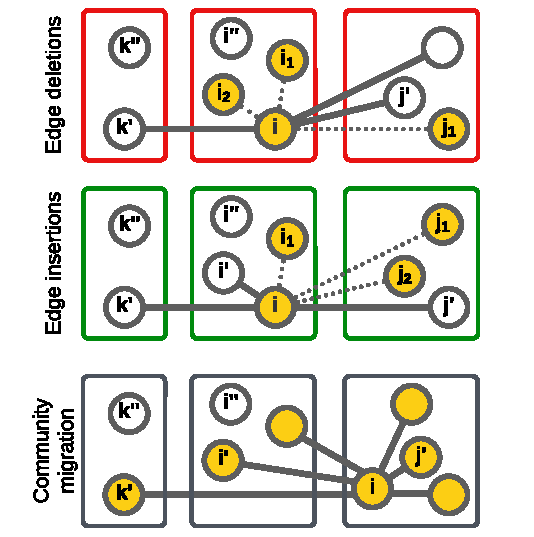
\includegraphics[width=0.78\linewidth]{out/about-frontier-detail.pdf}
  } \\[-2ex]
  \caption{A detailed illustration for presenting arguments on the correctness of \textit{Dynamic Frontier (DF)} Louvain.}
  \label{fig:frontier-approach}
\end{figure}





\subsubsection{On edge deletion}

\begin{lemma}
\label{thm:louvain--mark-deletion}
Given an edge deletion $(i, j)$ between vertices $i$ and $j$ belonging to the same community $d$, vertex $i$ (and $j$) should be marked as affected.
\end{lemma}

Consider the case of edge deletion $(i, j)$ of weight $w$ between vertices $i$ and $j$ belonging to the same community $C_i = C_j = d$ (see Figure \ref{fig:frontier-approach}, where $j = i_1$). Let $i''$ be a vertex belonging $i$'s community $C_{i''} = d$, and let $k''$ be a vertex belonging to another community $C_{k''} = b$. As shown below in Case \textbf{(1)}, the delta-modularity of vertex $i$ moving from its original community $d$ to another community $b$ has a significant positive factor $w/m$. There is thus a chance that vertex $i$ would change its community membership, and we should mark it as affected. The same argument applies for vertex $j$, as the edge is undirected. On the other hand, for the Cases \textbf{(2)}-\textbf{(3)}, there is only a small positive change in delta-modularity for vertex $k''$. Thus, there is little incentive for vertex $k''$ to change its community membership, and no incentive for a change in community membership of vertex $i''$.

Note that it is possible that the community $d$ would split due to the edge deletion. However, this is unlikely, given that one would need a large number of edge deletions between vertices belonging to the same community for the community to split. One can take care of such rare events by running Static Louvain, say every $1000$ batch updates, which also helps us ensure high-quality communities. The same applies to Delta-screening (DS) Louvain.

\begin{enumerate}
  \item $\Delta Q_{i:d \rightarrow b}^{new} = \Delta Q_{i:d \rightarrow b} + [\frac{w}{m}] + \frac{w}{2m^2} (\Sigma_c - \Sigma_d + w)$
  \item $\Delta Q_{i'':d \rightarrow b}^{new} = \Delta Q_{i'':d \rightarrow b} - \frac{wK_{i''}}{m^2}$
  \item $\Delta Q_{k'':b \rightarrow d}^{new} = \Delta Q_{k'':b \rightarrow d} + \frac{wK_{k''}}{m^2}$
\end{enumerate}

Now, consider the case of edge deletion $(i, j)$ between vertices $i$ and $j$ belonging to different communities, i.e., $C_i = d$, $C_j = c$ (see Figure \ref{fig:frontier-approach}, where $j = j_2$ or $j_3$). Let $i''$ be a vertex belonging to $i$'s community $C_{i''} = d$, $j''$ be a vertex belonging to $j$'s community $C_{j''} = c$, and $k''$ be a vertex belonging another community $C_{k''} = b$. As shown in Cases \textbf{(4)}-\textbf{(8)}, due to the absence of any significant positive change in delta-modularity, there is little to no incentive for vertices $i$, $j$, $k''$, $i''$, and $j''$ to change their community membership.

\begin{enumerate}[start=4]
  \item $\Delta Q_{i:d \rightarrow c}^{new} = \Delta Q_{i:d \rightarrow c} - \frac{w}{m} + \frac{w}{2m^2} (2K_i + \Sigma_c - \Sigma_d - w)$
  \item $\Delta Q_{i:d \rightarrow b}^{new} = \Delta Q_{i:d \rightarrow b} + \frac{w}{2m^2} (K_i + \Sigma_b - \Sigma_d)$
  \item $\Delta Q_{i'':d \rightarrow c}^{new} = \Delta Q_{i'':d \rightarrow c}$
  \item $\Delta Q_{i'':d \rightarrow b}^{new} = \Delta Q_{i'':d \rightarrow b} - \frac{wK_{i''}}{2m^2}$
  \item $\Delta Q_{k'':b \rightarrow d/c}^{new} = \Delta Q_{k'':b \rightarrow d/c} + \frac{wK_{k''}}{m^2}$ \hfill $\diamond$
\end{enumerate}




\subsubsection{On edge insertion}

\begin{lemma}
\label{thm:louvain--mark-insertion}
Given an edge insertion $(i, j, w)$ between vertices $i$ and $j$ belonging to different communities $d$ and $c$, vertex $i$ (and $j$) should be marked as affected.
\end{lemma}

Let us consider the case of edge insertion $(i, j, w)$ between vertices $i$ and $j$ belonging to different communities $C_i = d$ and $C_j = c$ respectively (see Figure \ref{fig:frontier-approach}, where $j = j_3$). Let $i''$ be a vertex belonging $i$'s community $C_{i''} = d$, $j''$ be a vertex belonging to $j$'s community $C_{j''} = c$, and $k''$ be a vertex belonging to another community $C_{k''} = b$. As shown below in Case \textbf{(9)}, we have a significant positive factor $w/m$ (and a small negative factor) which increases the delta-modularity of vertex $i$ moving to $j$'s community after the insertion of the edge $(i, j)$. There is, therefore, incentive for vertex $i$ to change its community membership. Accordingly, we mark $i$ as affected. Again, the same argument applies for vertex $j$, as the edge is undirected. Further, we observe from other Cases \textbf{(10)}-\textbf{(13)} there is only a small change in delta-modularity. Thus, there is hardly any to no incentive for a change in community membership of vertices $i''$, $j''$, and $k''$.

\begin{enumerate}[start=9]
  \item $\Delta Q_{i:d \rightarrow c}^{new} = \Delta Q_{i:d \rightarrow c} + [\frac{w}{m}] - \frac{w}{2m^2} (2K_i + \Sigma_c - \Sigma_d + w)$
  \item $\Delta Q_{i:d \rightarrow b}^{new} = \Delta Q_{i:d \rightarrow b} - \frac{w}{2m^2} (K_i + \Sigma_b - \Sigma_d)$
  \item $\Delta Q_{i'':d \rightarrow c}^{new} = \Delta Q_{i'':d \rightarrow c}$
  \item $\Delta Q_{i'':d \rightarrow b}^{new} = \Delta Q_{i'':d \rightarrow b} + \frac{wK_{i''}}{2m^2}$
  \item $\Delta Q_{k'':b \rightarrow d/c}^{new} = \Delta Q_{k'':b \rightarrow d/c} - \frac{wK_{k''}}{2m^2}$
\end{enumerate}

Now, consider the case of edge insertion $(i, j, w)$ between vertices $i$ and $j$ belonging to the same community $C_i = C_j = d$ (see Figure \ref{fig:frontier-approach}, where $j = i_1$ or $i_2$). From Cases \textbf{(14)}-\textbf{(16)}, we note that it is little to no incentive for vertices $i''$, $k''$, $i$, and $j$ to change their community membership. Note that it is possible for the insertion of edges within the same community to cause it to split into two more strongly connected communities, but it is very unlikely.

\begin{enumerate}[start=14]
  \item $\Delta Q_{i:d \rightarrow b}^{new} = \Delta Q_{i:d \rightarrow b} - \frac{w}{m} - \frac{w}{2m^2} (\Sigma_c - \Sigma_d - w)$
  \item $\Delta Q_{i'':d \rightarrow b}^{new} = \Delta Q_{i'':d \rightarrow b} + \frac{wK_{i''}}{m^2}$
  \item $\Delta Q_{k'':b \rightarrow d}^{new} = \Delta Q_{k'':b \rightarrow d} - \frac{wK_{k''}}{m^2}$ \hfill $\diamond$
\end{enumerate}




\subsubsection{On vertex migration to another community}

\begin{lemma}
\label{thm:louvain--remark}
When a vertex $i$ changes its community membership, and vertex $j$ is its neighbor, $j$ should be marked as affected.
\end{lemma}

We considered the direct effects of deletion and insertion of edges above. Now we consider its indirect effects by studying the impact of change in community membership of one vertex on the other vertices. Consider the case where a vertex $i$ changes its community membership from its previous community $d$ to a new community $c$ (see Figure \ref{fig:frontier-approach}). Let $i'$ be a neighbor of $i$ and $i''$ be a non-neighbor of $i$ belonging to $i$'s previous community $C_{i'} = C_{i''} = d$, $j'$ be a neighbor of $i$ and $j''$ be a non-neighbor of $i$ belonging to $i$'s new community $C_{j'} = C_{j''} = c$, $k'$ be a neighbor of $i$ and $k''$ be a non-neighbor of $i$ belonging to another community $C_{k'} = C_{k''} = b$. From Cases \textbf{(17)}-\textbf{(22)}, we note that neighbors $i'$ and $k'$ have an incentive to change their community membership (as thus necessitate marking), but not $j'$. However, to keep the algorithm simple, we simply mark all the neighbors of vertex $i$ as affected.

\begin{enumerate}[start=17]
  \item $\Delta Q_{i':d \rightarrow c}^{new} = \Delta Q_{i':d \rightarrow c} + [\frac{2w_{ii'}}{m}] - \frac{K_iK_{i'}}{m^2}$
  \item $\Delta Q_{i':d \rightarrow b}^{new} = \Delta Q_{i':d \rightarrow b} + [\frac{w_{ii'}}{m}] - \frac{K_iK_{i'}}{2m^2}$
  \item $\Delta Q_{j':c \rightarrow d}^{new} = \Delta Q_{j':c \rightarrow d} - \frac{2w_{ij'}}{m} + \frac{K_iK_{j'}}{m^2}$
  \item $\Delta Q_{j':c \rightarrow b}^{new} = \Delta Q_{j':c \rightarrow b} - \frac{w_{ij'}}{m} + \frac{K_iK_{j'}}{2m^2}$
  \item $\Delta Q_{k':b \rightarrow d}^{new} = \Delta Q_{k':b \rightarrow d} - \frac{w_{ik'}}{m} + \frac{K_iK_{k'}}{2m^2}$
  \item $\Delta Q_{k':b \rightarrow c}^{new} = \Delta Q_{k':b \rightarrow c} + [\frac{w_{ik'}}{m}] - \frac{K_iK_{k'}}{2m^2}$
\end{enumerate}

Further, from Cases \textbf{(23)}-\textbf{(28)}, we note that there is hardly any incentive for a change in community membership of vertices $i''$, $j''$, and $k''$. This is due to the change in delta-modularity being insignificant. There could still be an indirect cascading impact, where a common neighbor between vertices $i$ and $j$ would change its community, which could eventually cause vertex $j$ to change its community as well \cite{com-zarayeneh21}. However, this case is automatically taken care of as we perform marking of affected vertices during the community detection process.

\begin{enumerate}[start=23]
  \item $\Delta Q_{i'':d \rightarrow c}^{new} = \Delta Q_{i'':d \rightarrow c} + \frac{K_iK_{i''}}{m^2}$
  \item $\Delta Q_{i'':d \rightarrow b}^{new} = \Delta Q_{i'':d \rightarrow b} - \frac{K_iK_{i''}}{2m^2}$
  \item $\Delta Q_{j'':c \rightarrow d}^{new} = \Delta Q_{j'':c \rightarrow d} + \frac{K_iK_{j''}}{m^2}$
  \item $\Delta Q_{j'':c \rightarrow b}^{new} = \Delta Q_{j'':c \rightarrow b} + \frac{K_iK_{j''}}{2m^2}$
  \item $\Delta Q_{k'':b \rightarrow d}^{new} = \Delta Q_{k'':b \rightarrow d} + \frac{K_iK_{k''}}{2m^2}$
  \item $\Delta Q_{k'':b \rightarrow c}^{new} = \Delta Q_{k'':b \rightarrow c} - \frac{K_iK_{k''}}{2m^2}$ \hfill $\diamond$
\end{enumerate}




\subsubsection{Overall}

Finally, based on Observations \ref{thm:louvain--mark-deletion}, \ref{thm:louvain--mark-insertion}, and \ref{thm:louvain--remark}, we can state the following for DF Louvain.

\begin{theorem}
\label{thm:louvain}
Given a batch update, DF Louvain marks vertices having an incentive to change their community\ignore{membership} as affected. \qed
\end{theorem}

We note that with DF Louvain, without any direct link to vertices in the frontier, outlier vertices may not be marked as affected --- even if they have the potential to change community. Such outliers may be weakly connected to multiple communities, and if the current community becomes weakly (or less strongly) connected, they may leave and join some other community. It may also be noted that DS Louvain is also an approximate method and can miss certain outliers. In practice, however, we see little to no impact of this approximation of the affected subset of the graph on the final quality (modularity) of the communities obtained, as shown in Section \ref{sec:evaluation}.




\begin{figure*}[!hbt]
  \centering
  \subfigure[Runtime on consecutive batch updates of size $10^{-5}|E_T|$]{
    \label{fig:temporal-sx-mathoverflow--runtime5}
    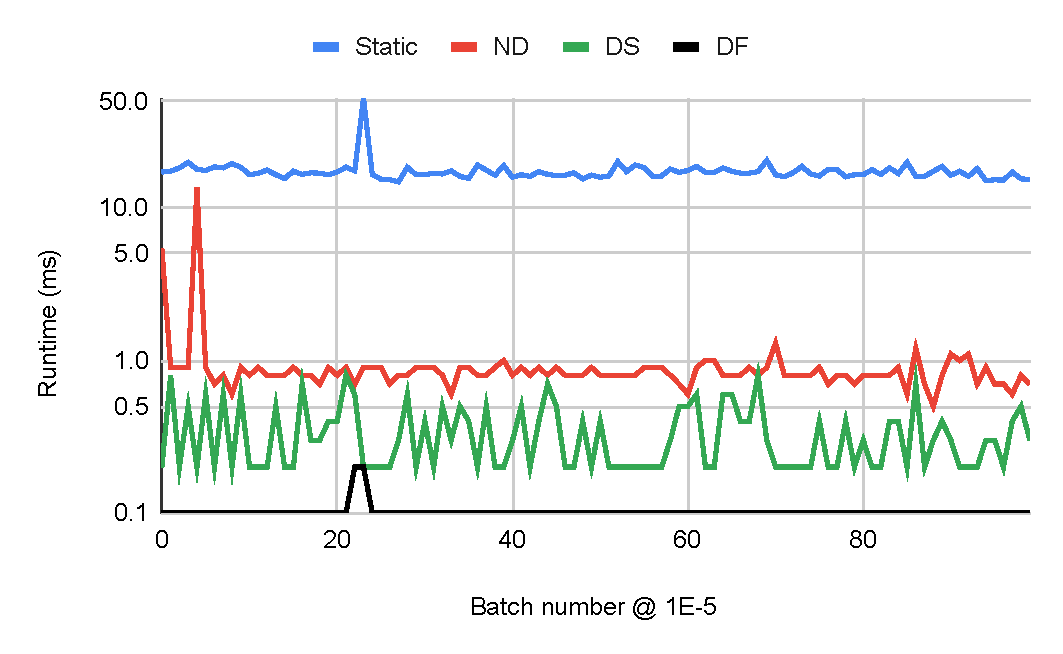
\includegraphics[width=0.48\linewidth]{out/temporal-sx-mathoverflow-runtime5.pdf}
  }
  \subfigure[Modularity in ranks obtained on consecutive batch updates of size $10^{-5}|E_T|$]{
    \label{fig:temporal-sx-mathoverflow--modularity5}
    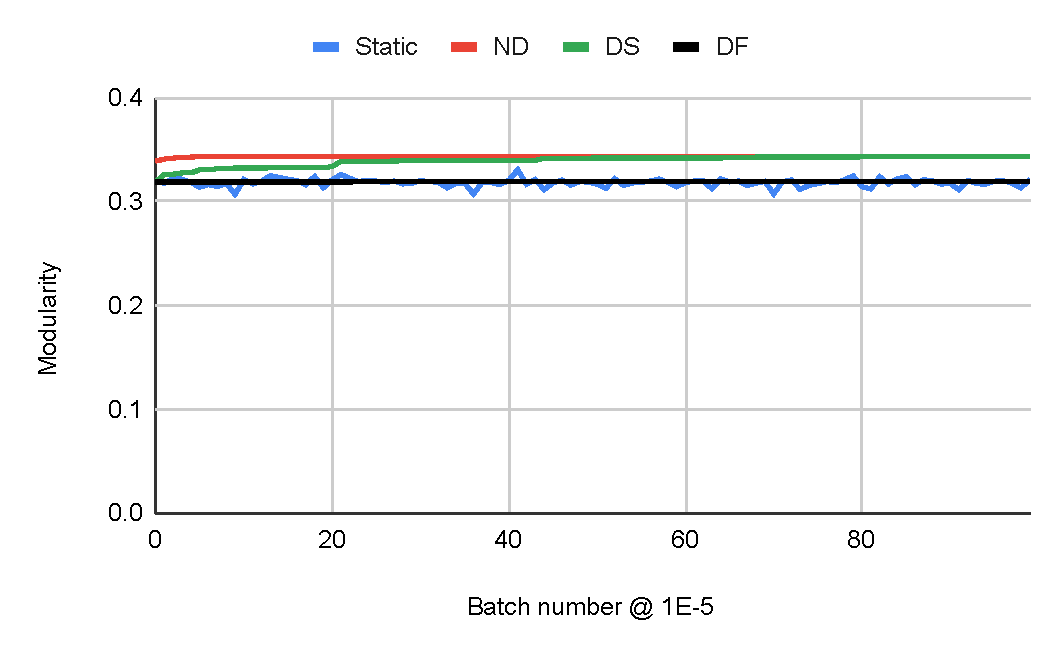
\includegraphics[width=0.48\linewidth]{out/temporal-sx-mathoverflow-modularity5.pdf}
  } \\[2ex]
  \subfigure[Runtime on consecutive batch updates of size $10^{-4}|E_T|$]{
    \label{fig:temporal-sx-mathoverflow--runtime4}
    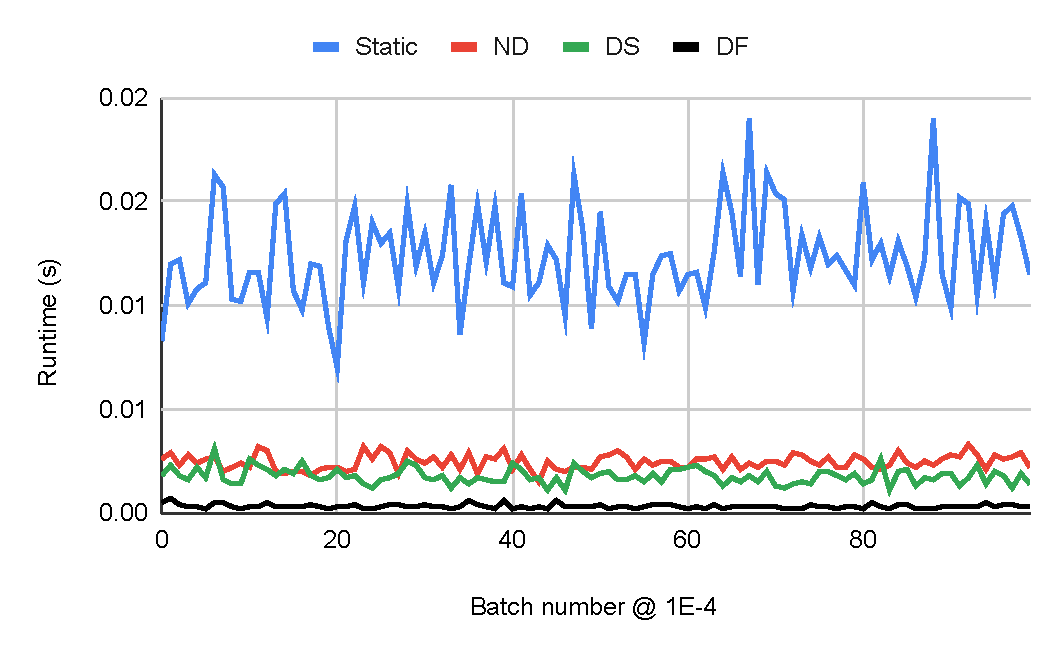
\includegraphics[width=0.48\linewidth]{out/temporal-sx-mathoverflow-runtime4.pdf}
  }
  \subfigure[Modularity in ranks obtained on consecutive batch updates of size $10^{-4}|E_T|$]{
    \label{fig:temporal-sx-mathoverflow--modularity4}
    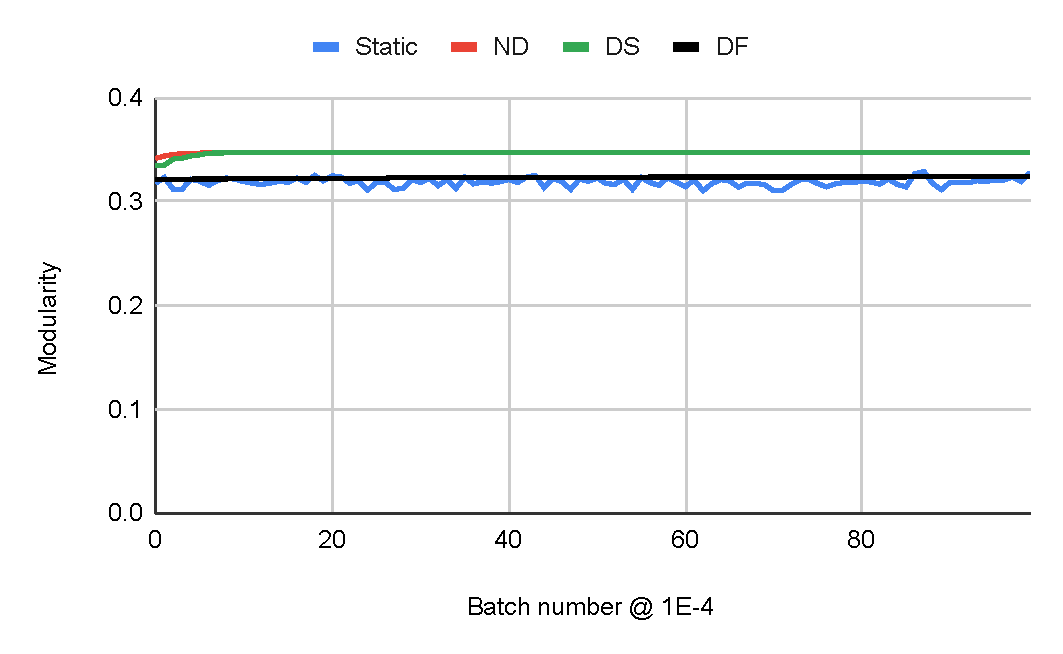
\includegraphics[width=0.48\linewidth]{out/temporal-sx-mathoverflow-modularity4.pdf}
  } \\[2ex]
  \subfigure[Runtime on consecutive batch updates of size $10^{-3}|E_T|$]{
    \label{fig:temporal-sx-mathoverflow--runtime3}
    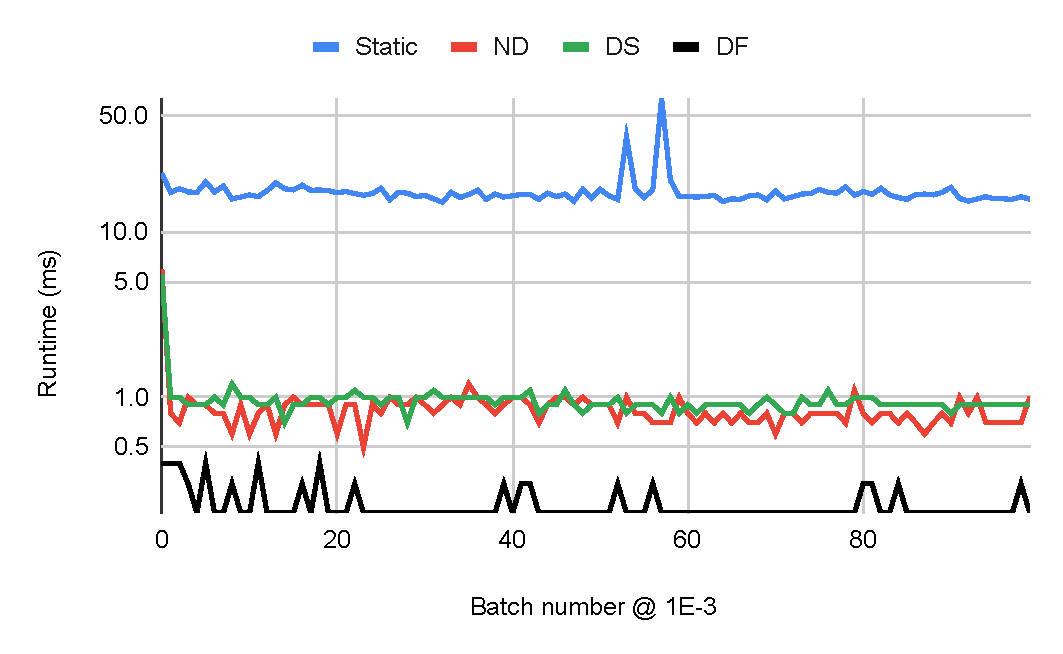
\includegraphics[width=0.48\linewidth]{out/temporal-sx-mathoverflow-runtime3.pdf}
  }
  \subfigure[Modularity in ranks obtained on consecutive batch updates of size $10^{-3}|E_T|$]{
    \label{fig:temporal-sx-mathoverflow--modularity3}
    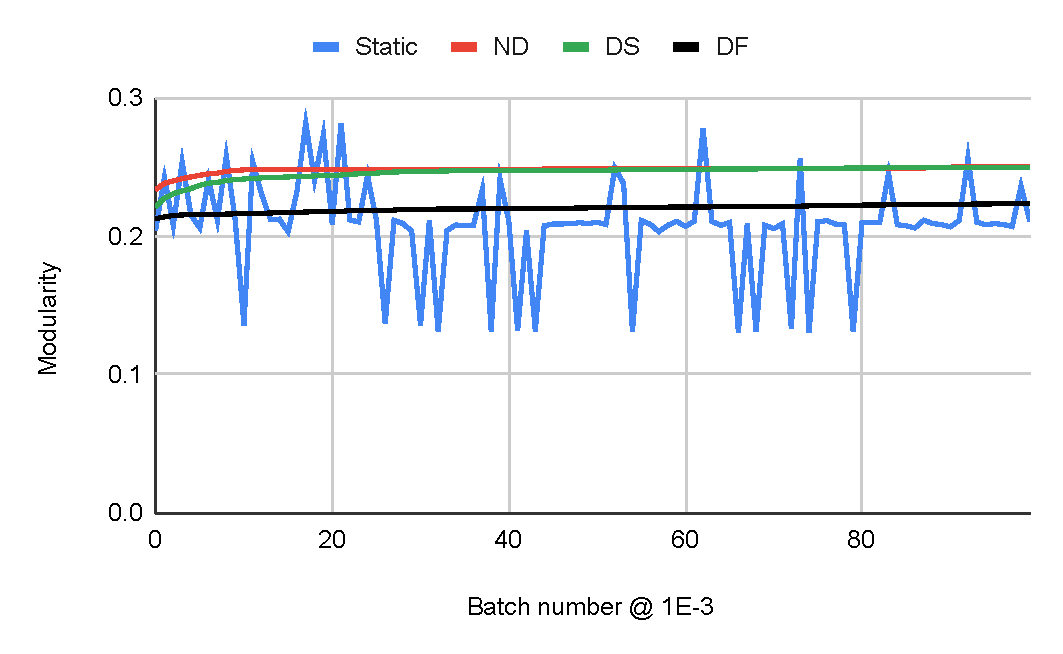
\includegraphics[width=0.48\linewidth]{out/temporal-sx-mathoverflow-modularity3.pdf}
  } \\[-2ex]
  \caption{Runtime and Modularity of communities obtained with our GPU implementation of \textit{Static}, \textit{Naive-dynamic (ND)}, \textit{Dynamic Traversal (DT)}, \textit{Dynamic Frontier (DF)}, and \textit{Dynamic Frontier with Pruning (DF-P)} PageRank on the \textit{sx-mathoverflow} dynamic graph. The size of batch updates range from $10^{-5}|E_T|$ to $10^{-3}|E_T|$. The rank modularity with each approach is measured relative to ranks obtained with a reference Static PageRank run, as detailed in Section \ref{sec:measurement}.}
  \label{fig:temporal-sx-mathoverflow}
\end{figure*}

\begin{figure*}[!hbt]
  \centering
  \subfigure[Runtime on consecutive batch updates of size $10^{-5}|E_T|$]{
    \label{fig:temporal-sx-askubuntu--runtime5}
    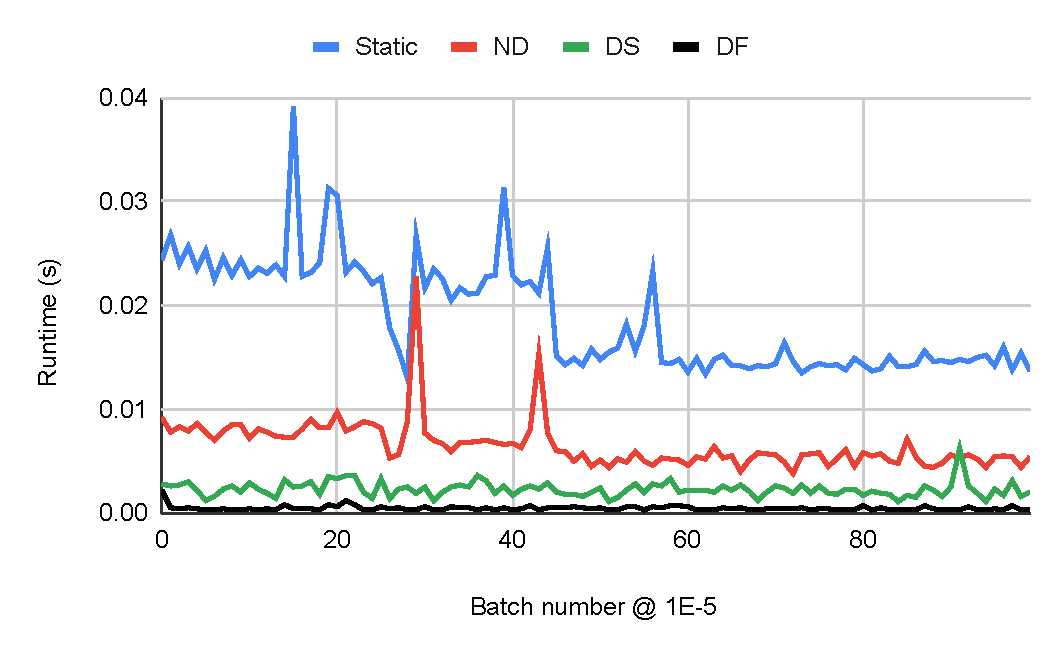
\includegraphics[width=0.48\linewidth]{out/temporal-sx-askubuntu-runtime5.pdf}
  }
  \subfigure[Modularity in ranks obtained on consecutive batch updates of size $10^{-5}|E_T|$]{
    \label{fig:temporal-sx-askubuntu--modularity5}
    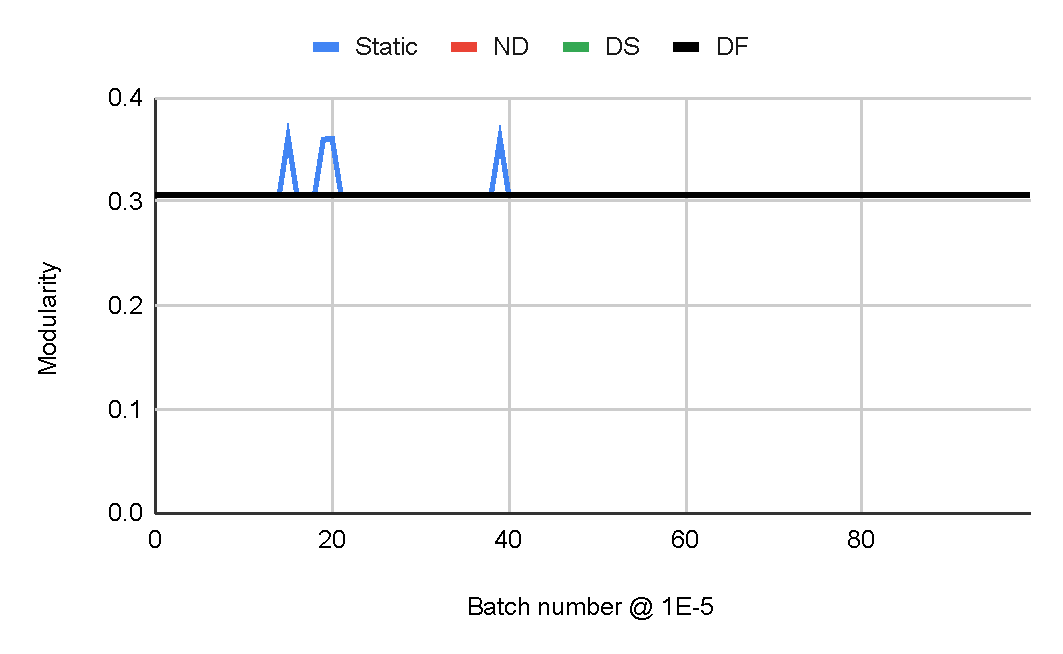
\includegraphics[width=0.48\linewidth]{out/temporal-sx-askubuntu-modularity5.pdf}
  } \\[2ex]
  \subfigure[Runtime on consecutive batch updates of size $10^{-4}|E_T|$]{
    \label{fig:temporal-sx-askubuntu--runtime4}
    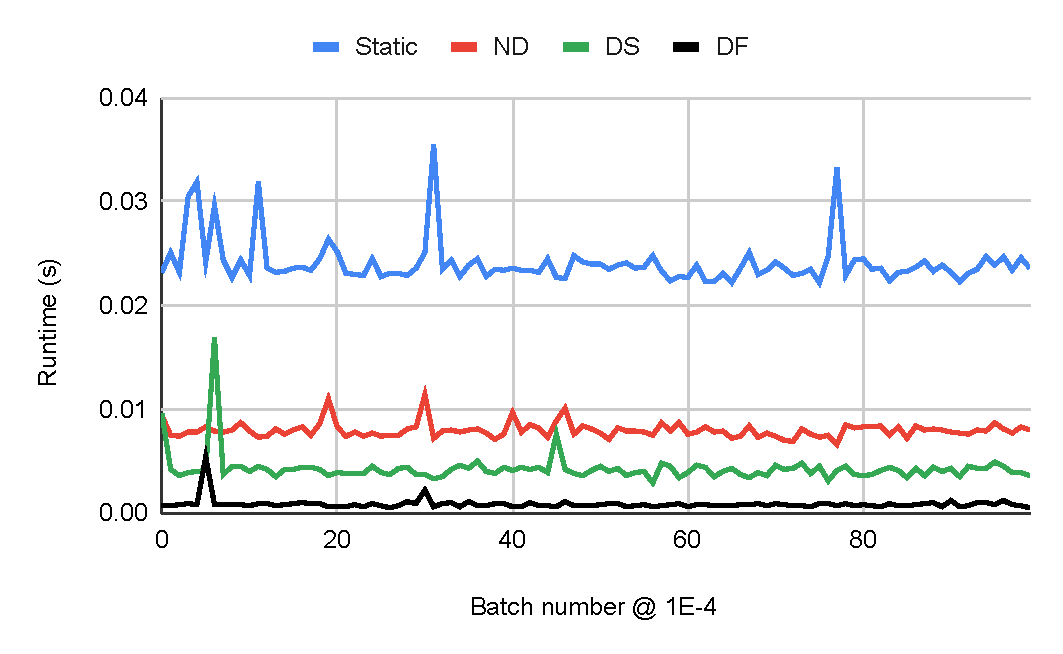
\includegraphics[width=0.48\linewidth]{out/temporal-sx-askubuntu-runtime4.pdf}
  }
  \subfigure[Modularity in ranks obtained on consecutive batch updates of size $10^{-4}|E_T|$]{
    \label{fig:temporal-sx-askubuntu--modularity4}
    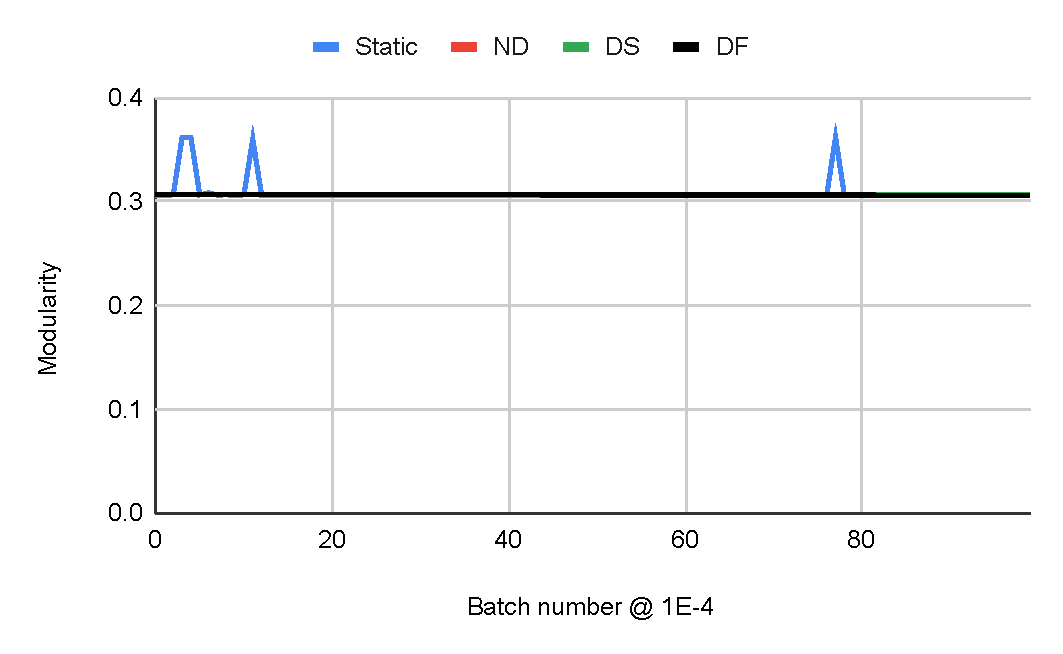
\includegraphics[width=0.48\linewidth]{out/temporal-sx-askubuntu-modularity4.pdf}
  } \\[2ex]
  \subfigure[Runtime on consecutive batch updates of size $10^{-3}|E_T|$]{
    \label{fig:temporal-sx-askubuntu--runtime3}
    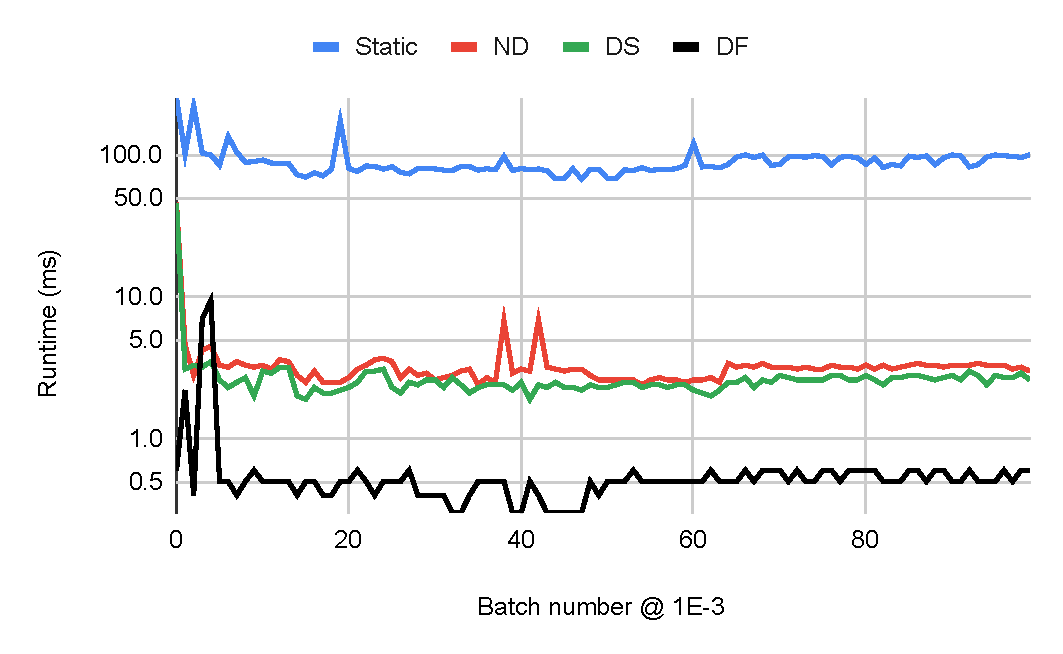
\includegraphics[width=0.48\linewidth]{out/temporal-sx-askubuntu-runtime3.pdf}
  }
  \subfigure[Modularity in ranks obtained on consecutive batch updates of size $10^{-3}|E_T|$]{
    \label{fig:temporal-sx-askubuntu--modularity3}
    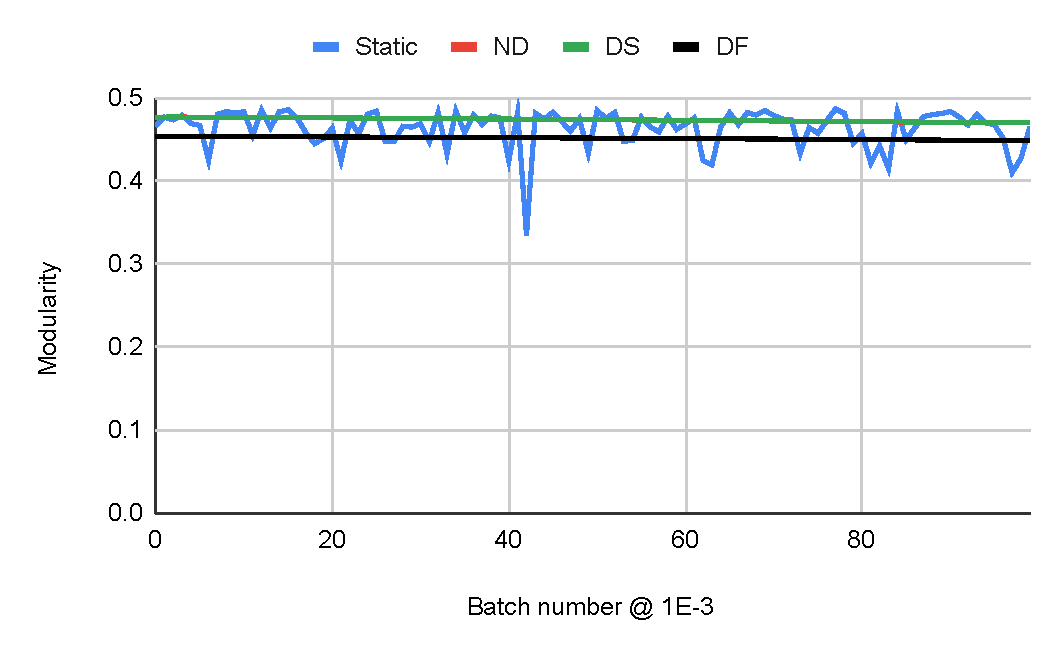
\includegraphics[width=0.48\linewidth]{out/temporal-sx-askubuntu-modularity3.pdf}
  } \\[-2ex]
  \caption{Runtime and Modularity of communities obtained with our GPU implementation of \textit{Static}, \textit{Naive-dynamic (ND)}, \textit{Dynamic Traversal (DT)}, \textit{Dynamic Frontier (DF)}, and \textit{Dynamic Frontier with Pruning (DF-P)} PageRank on the \textit{sx-askubuntu} dynamic graph. The size of batch updates range from $10^{-5}|E_T|$ to $10^{-3}|E_T|$. The rank modularity with each approach is measured relative to ranks obtained with a reference Static PageRank run, as detailed in Section \ref{sec:measurement}.}
  \label{fig:temporal-sx-askubuntu}
\end{figure*}

\begin{figure*}[!hbt]
  \centering
  \subfigure[Runtime on consecutive batch updates of size $10^{-5}|E_T|$]{
    \label{fig:temporal-sx-superuser--runtime5}
    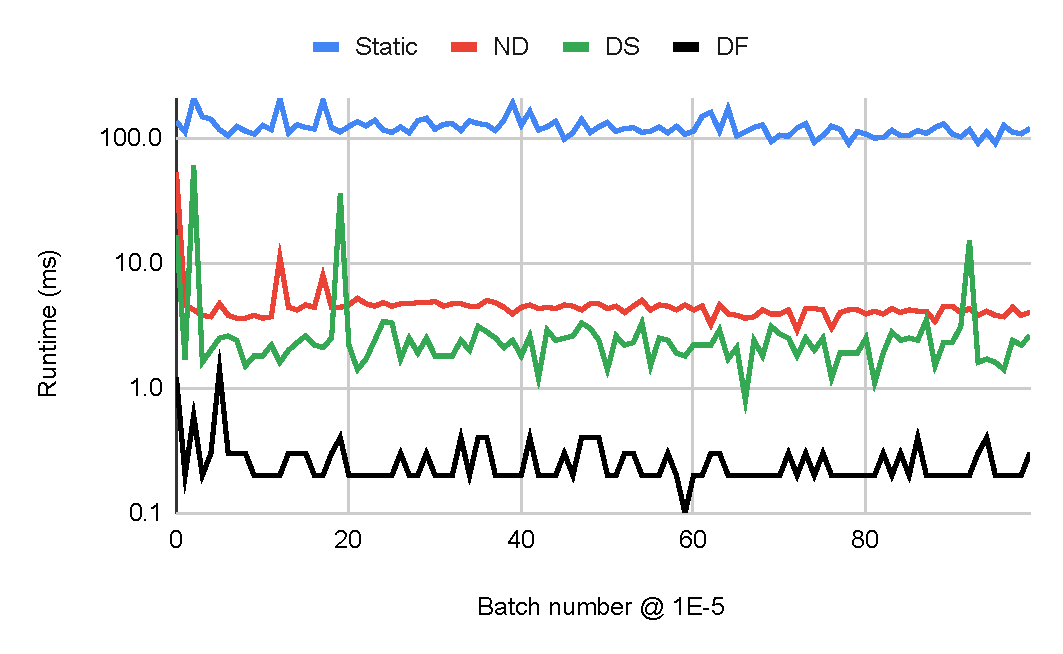
\includegraphics[width=0.48\linewidth]{out/temporal-sx-superuser-runtime5.pdf}
  }
  \subfigure[Modularity in ranks obtained on consecutive batch updates of size $10^{-5}|E_T|$]{
    \label{fig:temporal-sx-superuser--modularity5}
    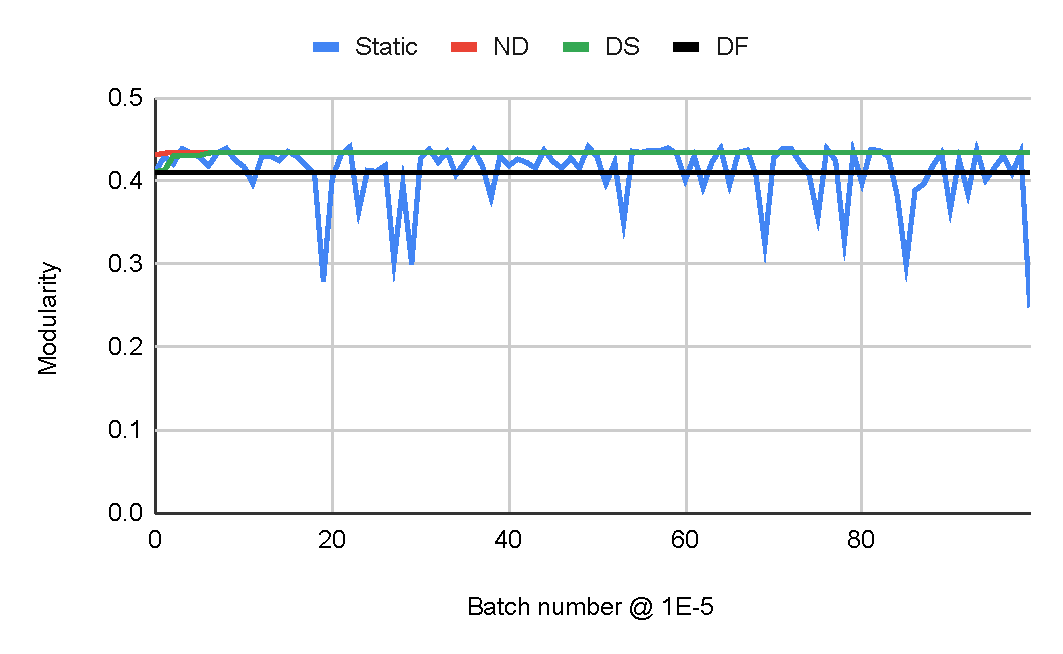
\includegraphics[width=0.48\linewidth]{out/temporal-sx-superuser-modularity5.pdf}
  } \\[2ex]
  \subfigure[Runtime on consecutive batch updates of size $10^{-4}|E_T|$]{
    \label{fig:temporal-sx-superuser--runtime4}
    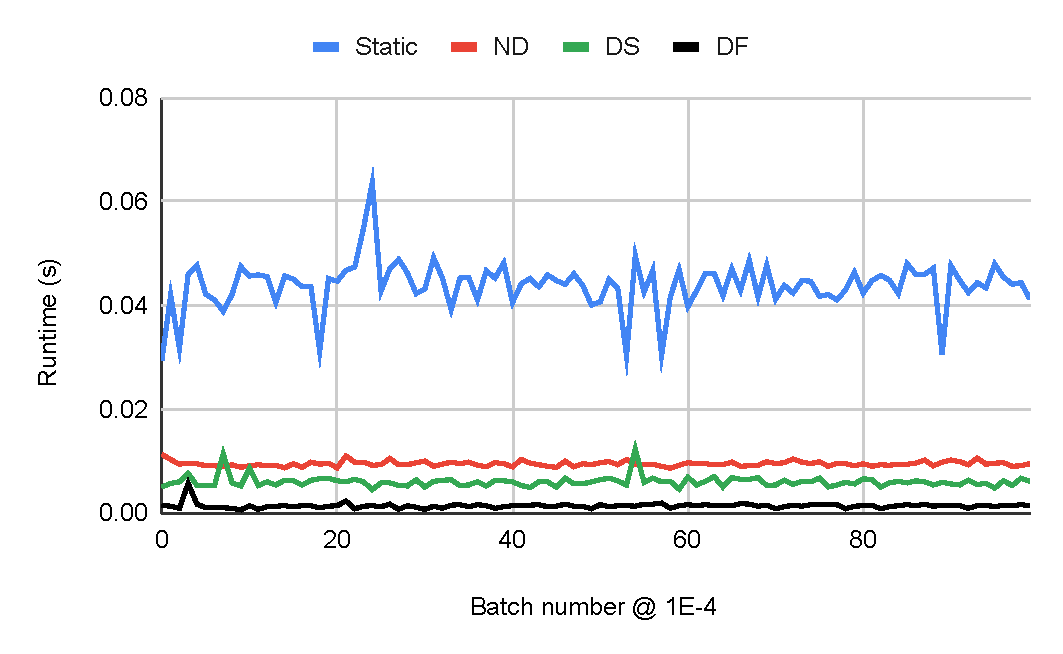
\includegraphics[width=0.48\linewidth]{out/temporal-sx-superuser-runtime4.pdf}
  }
  \subfigure[Modularity in ranks obtained on consecutive batch updates of size $10^{-4}|E_T|$]{
    \label{fig:temporal-sx-superuser--modularity4}
    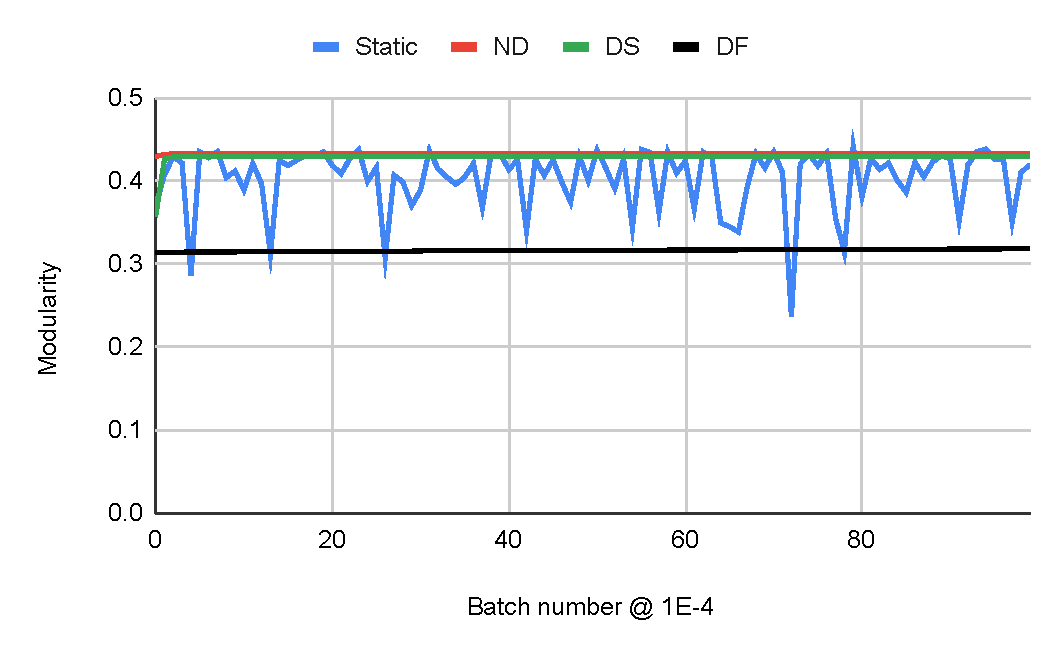
\includegraphics[width=0.48\linewidth]{out/temporal-sx-superuser-modularity4.pdf}
  } \\[2ex]
  \subfigure[Runtime on consecutive batch updates of size $10^{-3}|E_T|$]{
    \label{fig:temporal-sx-superuser--runtime3}
    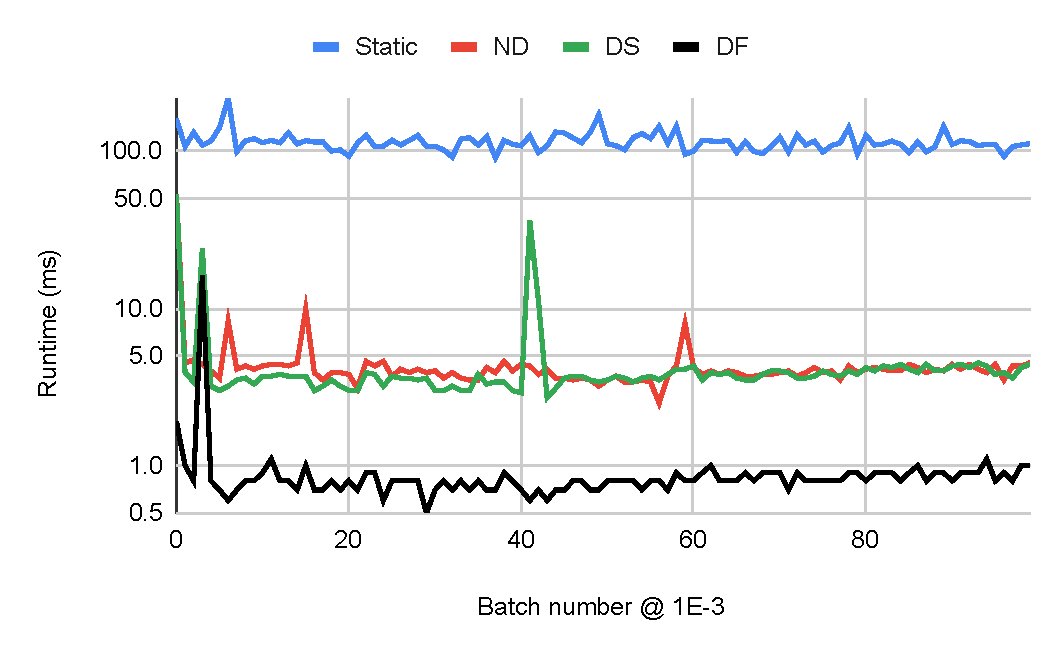
\includegraphics[width=0.48\linewidth]{out/temporal-sx-superuser-runtime3.pdf}
  }
  \subfigure[Modularity in ranks obtained on consecutive batch updates of size $10^{-3}|E_T|$]{
    \label{fig:temporal-sx-superuser--modularity3}
    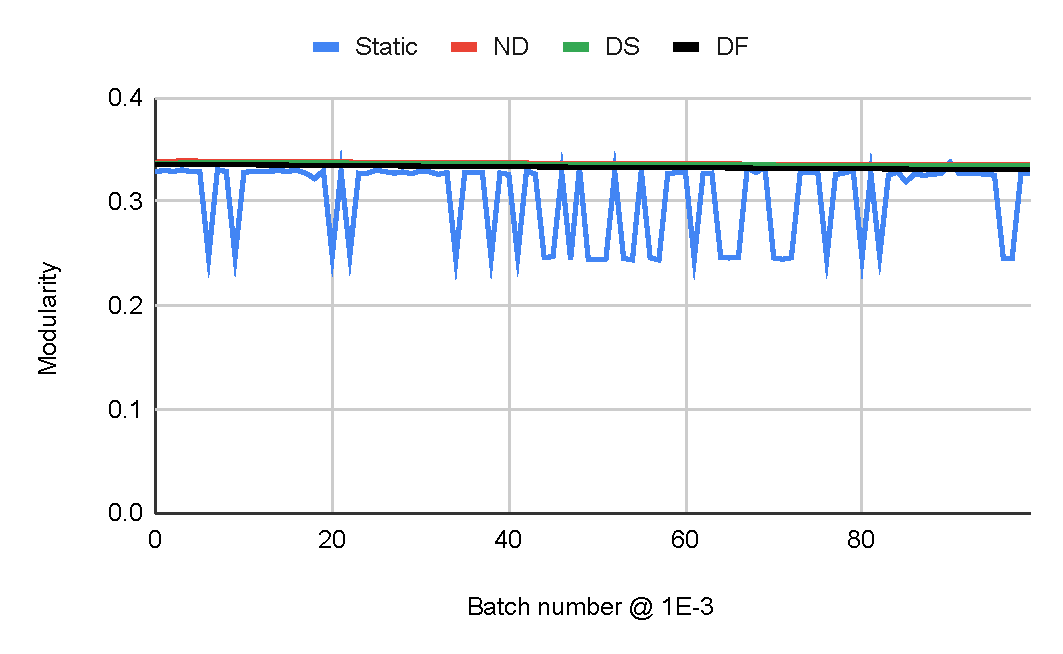
\includegraphics[width=0.48\linewidth]{out/temporal-sx-superuser-modularity3.pdf}
  } \\[-2ex]
  \caption{Runtime and Modularity of communities obtained with our GPU implementation of \textit{Static}, \textit{Naive-dynamic (ND)}, \textit{Dynamic Traversal (DT)}, \textit{Dynamic Frontier (DF)}, and \textit{Dynamic Frontier with Pruning (DF-P)} PageRank on the \textit{sx-superuser} dynamic graph. The size of batch updates range from $10^{-5}|E_T|$ to $10^{-3}|E_T|$. The rank modularity with each approach is measured relative to ranks obtained with a reference Static PageRank run, as detailed in Section \ref{sec:measurement}.}
  \label{fig:temporal-sx-superuser}
\end{figure*}

\begin{figure*}[!hbt]
  \centering
  \subfigure[Runtime on consecutive batch updates of size $10^{-5}|E_T|$]{
    \label{fig:temporal-wiki-talk-temporal--runtime5}
    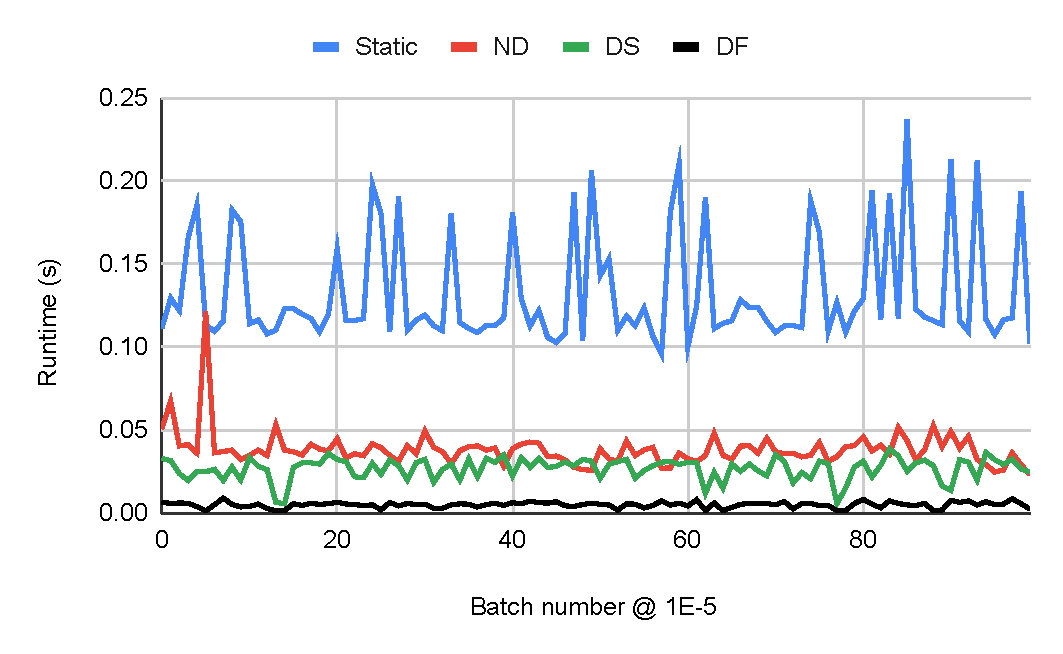
\includegraphics[width=0.48\linewidth]{out/temporal-wiki-talk-temporal-runtime5.pdf}
  }
  \subfigure[Modularity of communities obtained on consecutive batch updates of size $10^{-5}|E_T|$]{
    \label{fig:temporal-wiki-talk-temporal--modularity5}
    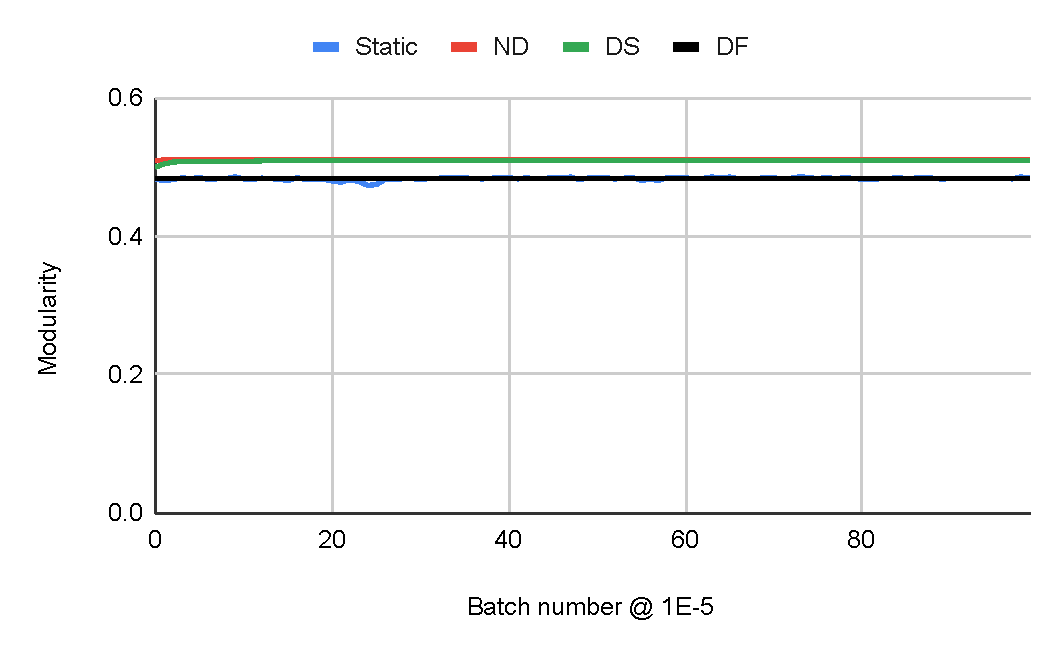
\includegraphics[width=0.48\linewidth]{out/temporal-wiki-talk-temporal-modularity5.pdf}
  } \\[2ex]
  \subfigure[Runtime on consecutive batch updates of size $10^{-4}|E_T|$]{
    \label{fig:temporal-wiki-talk-temporal--runtime4}
    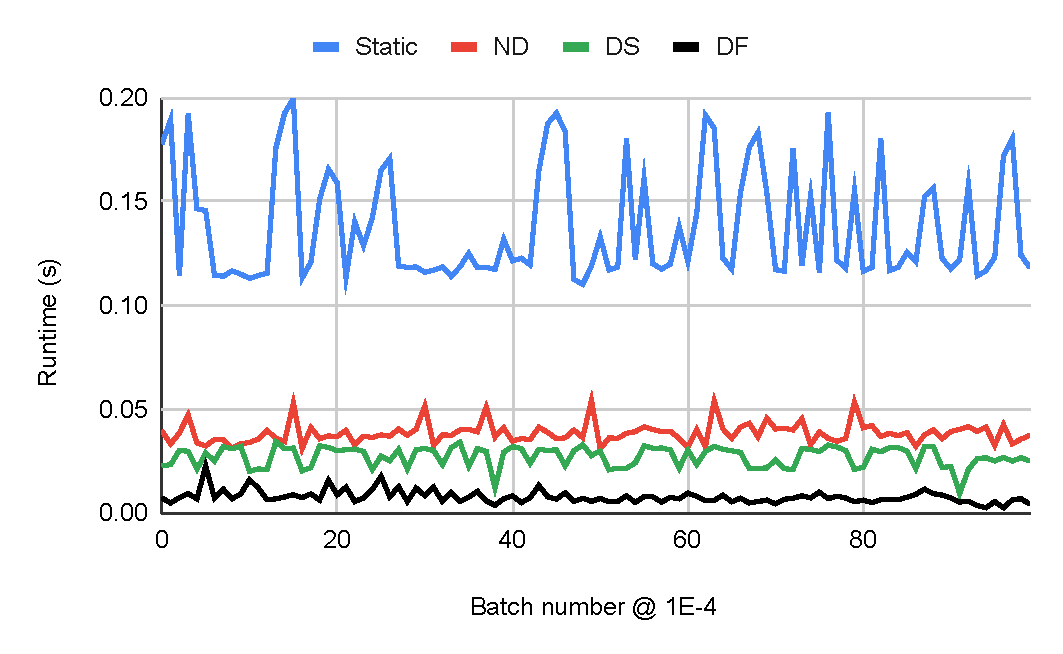
\includegraphics[width=0.48\linewidth]{out/temporal-wiki-talk-temporal-runtime4.pdf}
  }
  \subfigure[Modularity of communities obtained on consecutive batch updates of size $10^{-4}|E_T|$]{
    \label{fig:temporal-wiki-talk-temporal--modularity4}
    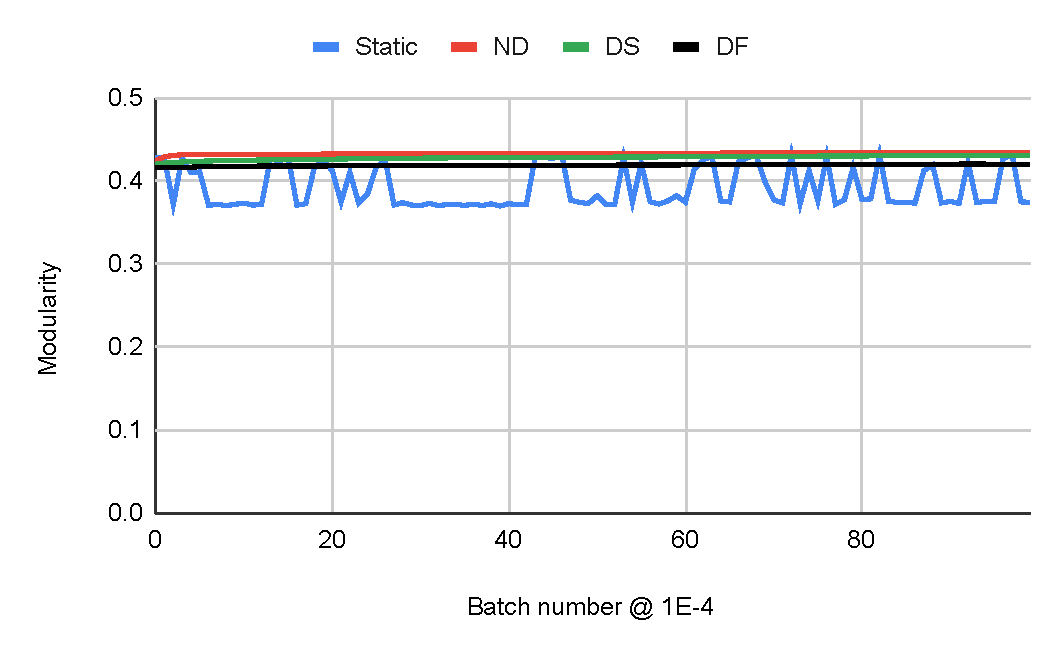
\includegraphics[width=0.48\linewidth]{out/temporal-wiki-talk-temporal-modularity4.pdf}
  } \\[2ex]
  \subfigure[Runtime on consecutive batch updates of size $10^{-3}|E_T|$]{
    \label{fig:temporal-wiki-talk-temporal--runtime3}
    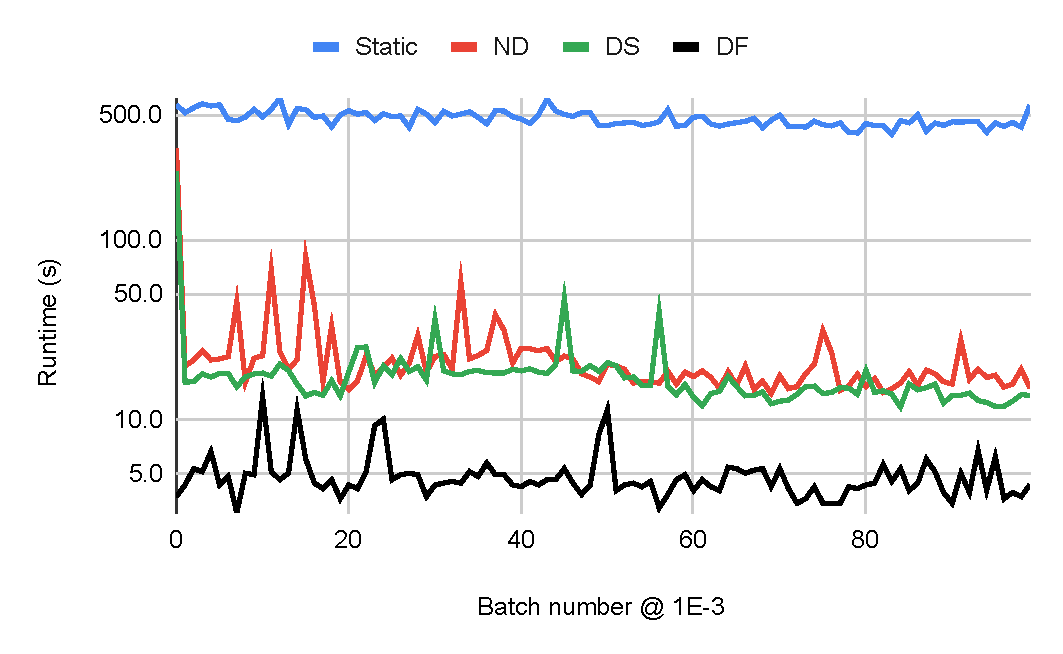
\includegraphics[width=0.48\linewidth]{out/temporal-wiki-talk-temporal-runtime3.pdf}
  }
  \subfigure[Modularity of communities obtained on consecutive batch updates of size $10^{-3}|E_T|$]{
    \label{fig:temporal-wiki-talk-temporal--modularity3}
    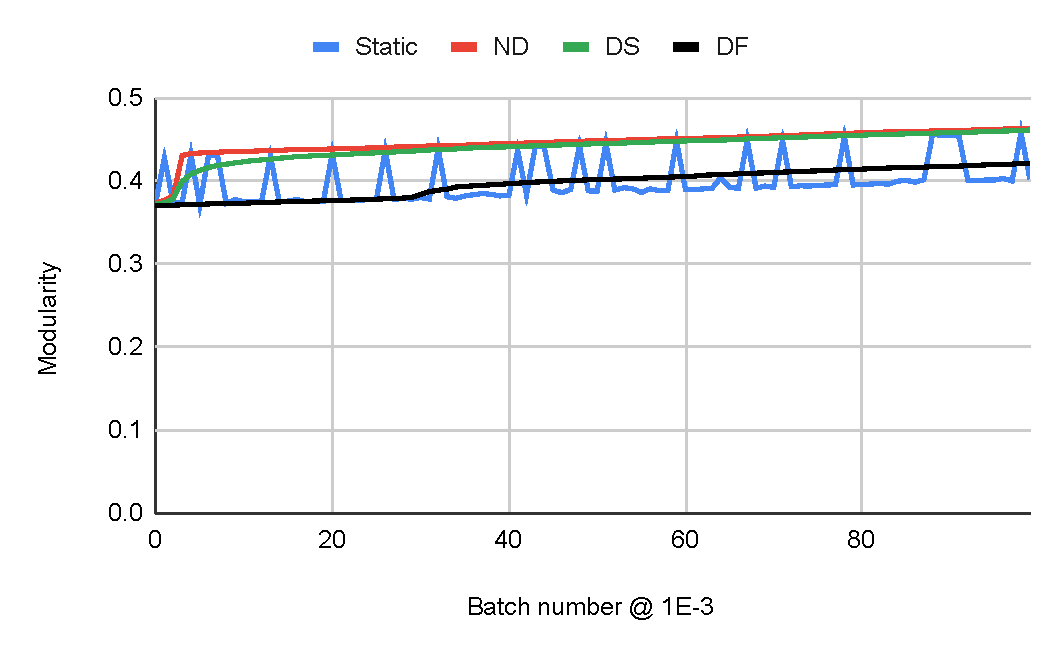
\includegraphics[width=0.48\linewidth]{out/temporal-wiki-talk-temporal-modularity3.pdf}
  } \\[-2ex]
  \caption{Runtime and Modularity of communities obtained with \textit{Static}, \textit{Naive-dynamic (ND)}, \textit{Delta-screening (DS)}, and \textit{Dynamic Frontier (DF)} Louvain on the \textit{wiki-talk-temporal} dynamic graph. The size of batch updates range from $10^{-5}|E_T|$ to $10^{-3}|E_T|$.}
  \label{fig:temporal-wiki-talk-temporal}
\end{figure*}

\begin{figure*}[!hbt]
  \centering
  \subfigure[Runtime on consecutive batch updates of size $10^{-5}|E_T|$]{
    \label{fig:temporal-sx-stackoverflow--runtime5}
    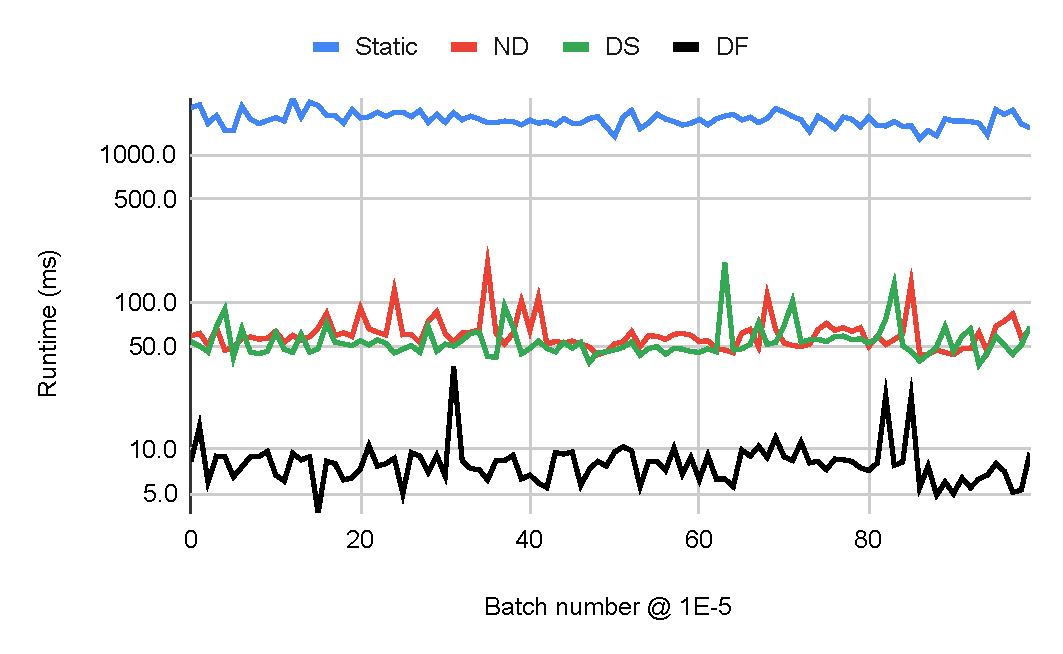
\includegraphics[width=0.48\linewidth]{out/temporal-sx-stackoverflow-runtime5.pdf}
  }
  \subfigure[Modularity in ranks obtained on consecutive batch updates of size $10^{-5}|E_T|$]{
    \label{fig:temporal-sx-stackoverflow--modularity5}
    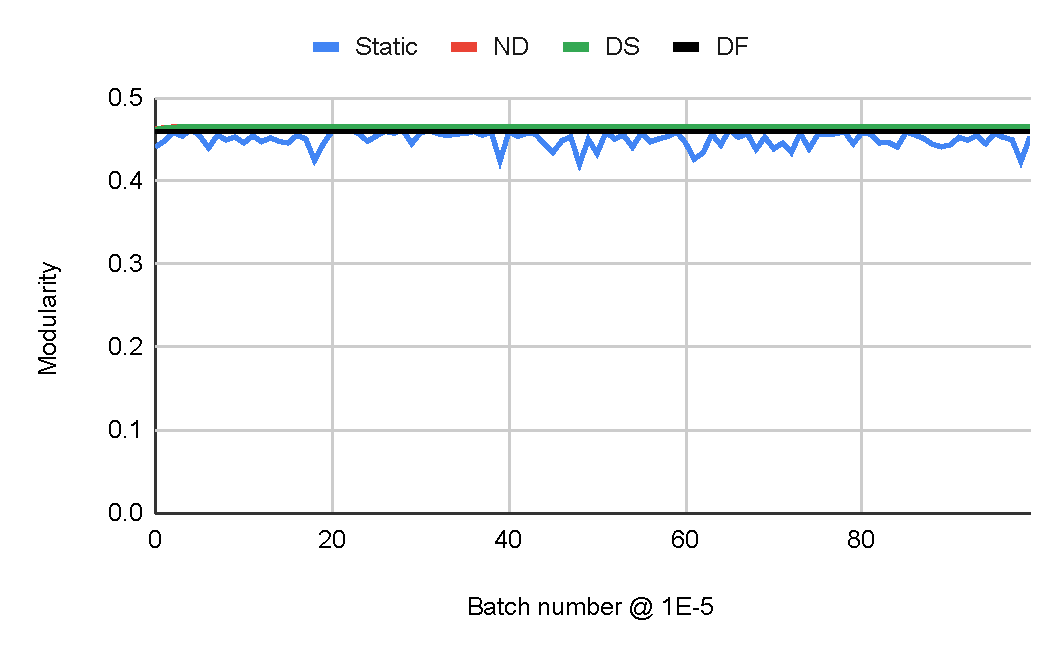
\includegraphics[width=0.48\linewidth]{out/temporal-sx-stackoverflow-modularity5.pdf}
  } \\[2ex]
  \subfigure[Runtime on consecutive batch updates of size $10^{-4}|E_T|$]{
    \label{fig:temporal-sx-stackoverflow--runtime4}
    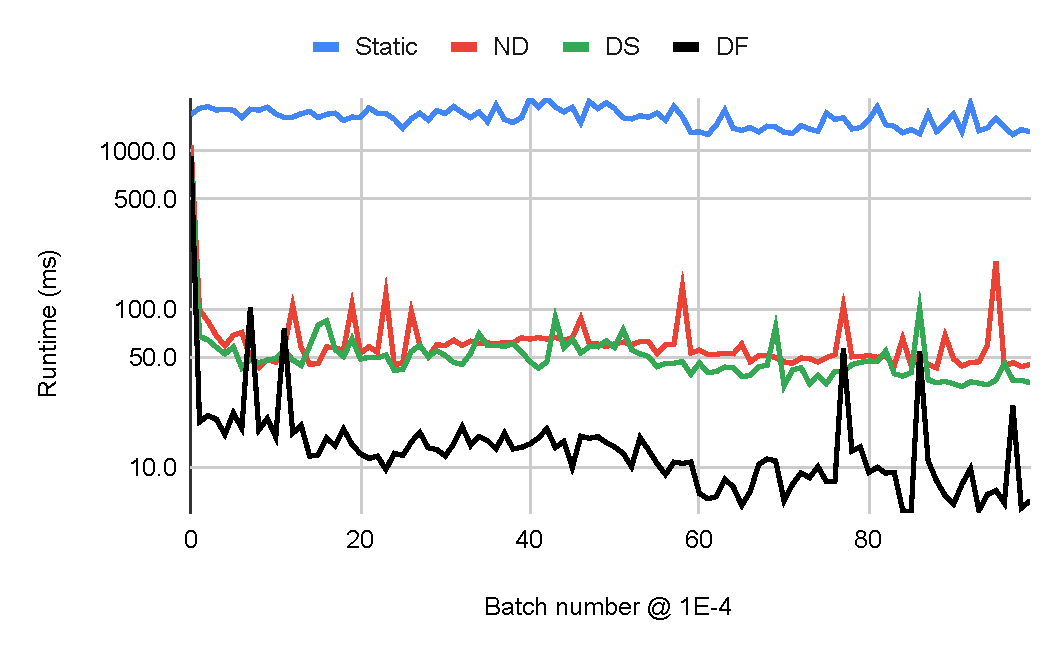
\includegraphics[width=0.48\linewidth]{out/temporal-sx-stackoverflow-runtime4.pdf}
  }
  \subfigure[Modularity in ranks obtained on consecutive batch updates of size $10^{-4}|E_T|$]{
    \label{fig:temporal-sx-stackoverflow--modularity4}
    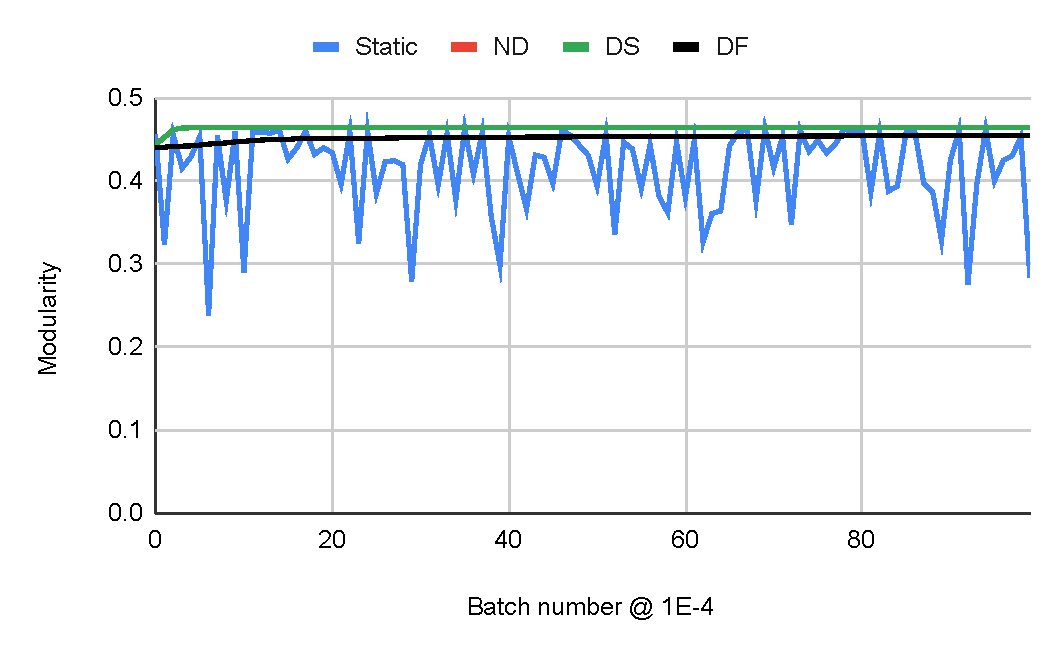
\includegraphics[width=0.48\linewidth]{out/temporal-sx-stackoverflow-modularity4.pdf}
  } \\[2ex]
  \subfigure[Runtime on consecutive batch updates of size $10^{-3}|E_T|$]{
    \label{fig:temporal-sx-stackoverflow--runtime3}
    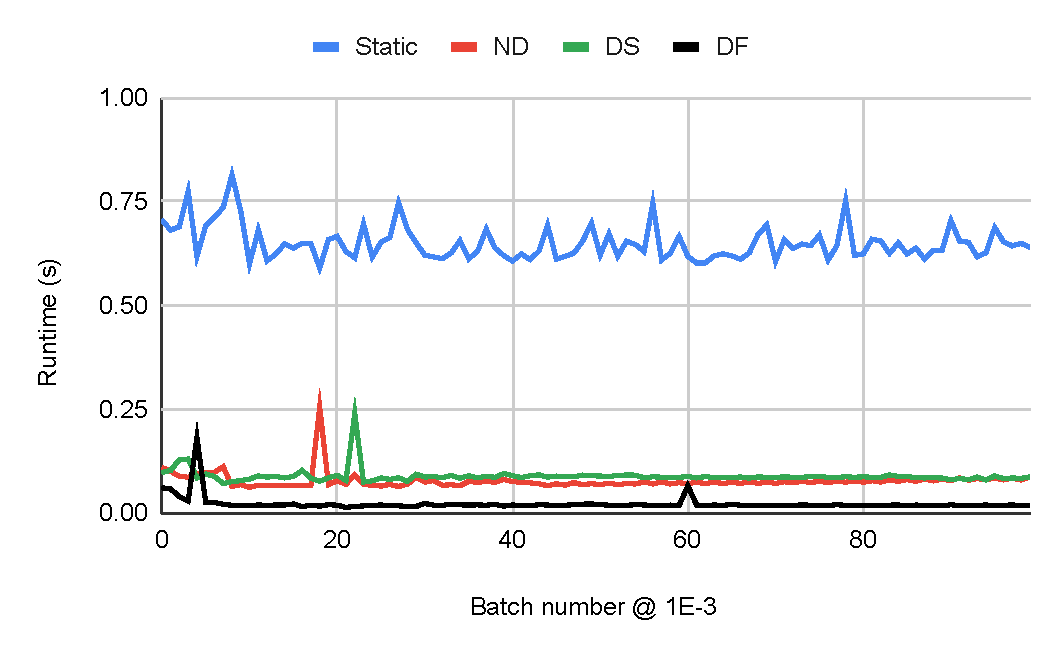
\includegraphics[width=0.48\linewidth]{out/temporal-sx-stackoverflow-runtime3.pdf}
  }
  \subfigure[Modularity in ranks obtained on consecutive batch updates of size $10^{-3}|E_T|$]{
    \label{fig:temporal-sx-stackoverflow--modularity3}
    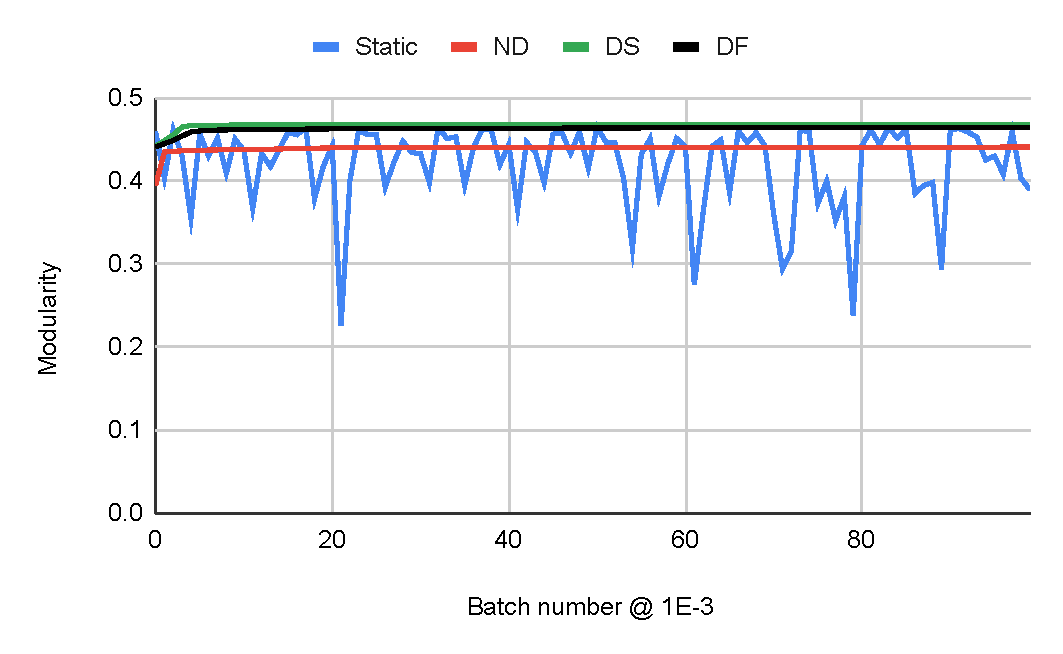
\includegraphics[width=0.48\linewidth]{out/temporal-sx-stackoverflow-modularity3.pdf}
  } \\[-2ex]
  \caption{Runtime and Modularity of communities obtained with our GPU implementation of \textit{Static}, \textit{Naive-dynamic (ND)}, \textit{Dynamic Traversal (DT)}, \textit{Dynamic Frontier (DF)}, and \textit{Dynamic Frontier with Pruning (DF-P)} PageRank on the \textit{sx-stackoverflow} dynamic graph. The size of batch updates range from $10^{-5}|E_T|$ to $10^{-3}|E_T|$. The rank modularity with each approach is measured relative to ranks obtained with a reference Static PageRank run, as detailed in Section \ref{sec:measurement}.}
  \label{fig:temporal-sx-stackoverflow}
\end{figure*}

